\documentclass[a4paper,12pt,titlepage]{article} % [papersize,fontsize,add title page]{document type}

% This LaTeX file can be turned straight into a pdf by "PDFTeXify" in WinEdit, or
% by any LaTeX --> PDF command in another LaTeX editor
%
% Because figure files are PDF, LaTeX --> DVI does not work

% usepackage{.} reads in additional LaTeX packages
\usepackage[pdftex]{graphicx}       % to include graphs
\usepackage{natbib}                % A BibTeX style file for references.
\usepackage{amssymb,amsmath}        % for maths symbols and equation numbering
\usepackage{array,tabularx,calc}
\usepackage{multirow} % create the tables
\usepackage{lscape} %put table lscape
\usepackage{pdflscape} %put pages lscape
\usepackage{listings}
\usepackage[T1]{fontenc}   %for the ""
\usepackage[title]{appendix} %for appendix

\newenvironment{conditions}[1][where:]
{%
	#1\tabularx{\textwidth-\widthof{#1}}[t]{
		>{$}l<{$} @{${}={}$} X@{}
	}%
}
{\endtabularx\\[\belowdisplayskip]}

% set up title page
\title{The NIR Corn Data Set}
\author{YZPH8 \vspace{2cm} \\
	Supervisor : Prof Tom Fearn \vspace{2cm} \\
	Department of Statistical Science \\
	University College London}
\date{\today} % \today gives today's date. ... or put in the date you want

% set page size and margins
\setlength{\textwidth}{17cm}
\setlength{\textheight}{26cm}
\setlength{\oddsidemargin}{-0.5cm}
\setlength{\evensidemargin}{-0.5cm}
\setlength{\topmargin}{-25mm}
\setlength{\parindent}{0cm}
\setlength{\parskip}{0.3cm}

\let\leq=\leqslant   % for nice-looking inequality signs
\let\geq=\geqslant

\numberwithin{equation}{section}  % equation numbers like (section#.equation#)

\linespread{1}     % 1: single-spacing, 2: double-spacing, 1.5: 1.5-spacing etc

\begin{document}   % start of document
	\maketitle         % create title etc
	
	\section{Abstruct} 
	
	One of the most easily accessible public data sets of high-dimensional NIR spectroscopic data is the so-called corn data. Its analysis has been reported in many publications, usually with the claim that some new method of data analysis performs better than the standard ones. The most common method of spectral analysis is partial least squares regression (PLSR). 
	
	First of all, the main job of this dissertation is to write a critical overview by reading as much literature as possible about corn data. Then summarize the patterns that affect PLSR. These patterns include pre-treatment, sample splitting,  number of samples, cross-validation and number of components. 
	
	Second, using the corn data to establish PLS model to research the specific impact of each patterns on the partial least squares regression results. Firstly, as the sample size increases, the prediction results of PLSR will get better and better and then tend to be stable or unstable but still keep better. Secondly, as the number of components increases, the prediction of PLSR will be better and better, and then worse. thirdly standardization is not a good pre-processing in the spectral analysis. Usually the effect of using the SavitzkyGolay filter will be better than not doing any pre-processing. Finally, the cross validation should be determined based on the original data. A k-fold cross validation is recommended when the sample data is too large.
	
	Moreover, select some papers that use corn data, and repeat the experiments in those papers to summarize the developed methods in papers. Analyze whether the difference between the developed methods and the standard method (PLS) is obvious and assess the developed methods made for improvements. Furthermore,  evaluate the difference between the developed methods and PLS, and construct an approximate F-statistics to detect whether the performance is significantly improved.
	
	last but not least, as part of dissertation, because there are too many dimensions to explore, and to ensure that the results are stable, it is necessary to perform a sufficient number of loop, which leads to a large amount of calculations in this dissertation. In order to solve the problem of computationly heavy, this dissertation first optimizes the code by modifying the program logic for parallel computing. Second, by submitting computing tasks to remote servers which is called the high performer computing system, a more stable computing environment and superior computer performance are achieved. Finally, because supercomputers have more cores than personal computers, parallel computing will play a bigger role on remote servers.
	\newpage           % start a new page
	
	\section{Acknowledgements} 
 I would like to thank my supervisor Professor Tom Fearn for his consistent support and guidance during this project. 
 
 I would also like to thank my parents and Chihyi CHANG for supporting me during the compilation of this dissertation. 
 

 Finally, I would also like to thank Dr. Chuling DING and Dr. Kevin Bronik for providing guidance about HPC. 
 
 
 	
 	
	\newpage           % start a new page
	
	\tableofcontents   % create table of contents
	\newpage           % start a new page
	

	
	\section{Introduction}             % start a new section called `Introduction'
	\label{sec:intro}                  % create label for this section
	
	Near-infrared spectroscopy is one of the spectral methods. Infrared spectroscopy combined with chemometric methods has been widely used in medical diagnostics, pharmaceuticals, food and various plant samples \citep{1su2006partial}. When the samples of plants are tested by near-infrared spectroscopy, this method is cheaper and faster than the conventional detection by chemical inspection methods. Since each wavelength in the spectrum corresponds to a compound bond, it is easy to judge the compound contained in a single compound by infrared spectroscopy. But the infrared spectrum has a wide range data. This results in a complex structure of the spectrum, so in many cases it is not possible to assign specific wavelength to specific chemical components. Therefore, a statistics method is needed to establish a prediction model in which spectral information is associated with sample eigenvalue. Because spectral information belongs to high dimension data and has strong multicollinearity, choosing an appropriate regression method is very important for prediction models. Multivariate regression analysis, such as principal component analysis (PCA), partial least squares regression (PLSR) or artificial neural networks, are often chosen to predict the required chemical information. Among those methods, PLSR has many applications in spectral analysis, and it is a very effective statistic method. The PLSR can not only comprehensively take out significant spectral data but also eliminate spectral multicollinearity problems. The main idea of algorithm is the multivariate statistical methods which reduce the dimensions of data, highlight the components, and then regression.
	
	The NIR spectroscopic data of corn is the most easily accessible high-dimensional public data set on the network. In recent years, many papers have analyzed corn data as an example. The most common algorithm for analyzing corn infrared spectral data is the PLSR. PLSR can effectively reduce the dimensionality of the infrared spectrum. This is one of the best ways at the moment. Therefore, a large part of the paper is based on the PLS method to improve the accuracy of the prediction. And this type of papers always claims that its method has better performance than PLS. Although this type of algorithm does show better performance from the results of the analysis, it should be noted that even the same corn NIR data set is analyzed. Different sampling methods, different principal component numbers, etc. will have an impact on the results. Most papers usually show that the new algorithm has smaller RMSECV and RMSEP than PLS. however only one regression result cannot judge the superiority of its model. And because some specific pre-processing, such as standardization, also makes a big difference in results.
	
	So the main work of this dissertation is to write a critical overview by reading as much literature as possible about corn data. And to find the commonly used options in the partial least squares model, such as different pre-treatment methods, different component selection methods, different cross-validation methods, and so on. These may affect the performance of the partial least squares regression model.
	And then to research the specific effects of each options on the partial least squares regression results based on corn data. This part usually uses the results of previous papers as a reference to ensure that the calculation process of dissertation is correct. 
	Finally, my results compares with the results in the papers and proposes a new method to test whether the new algorithm has better performance than PLSR. 
	
	Of course, as part of dissertation, because there are too many dimensions to explore, and to ensure that the results are stable, it is necessary to perform a sufficient number of loop, which leads to a large amount of calculations in this dissertation. In order to solve the problem of computationly heavy, this dissertation first optimizes the code by modifying the program logic for parallel computing. Second, by submitting computing tasks to remote servers which is called the high performer computing system, a more stable computing environment and superior computer performance are achieved. Finally, because supercomputers have more cores than personal computers, parallel computing will play a bigger role on remote servers.
	
	%\section{Literature reviews}
%	\label{sec:liter}
	
	\section{Datasets}
	\label{sec:data}
	
	Corn data is the most readily available high-dimensional Near-infrared spectral data. This data was published on the Internet (http://www.eigenvector.com/data/Corn/index.html) by Eigenvector Research, Inc. in 2005. The data consisted of 80 corn samples measured on three different NIR spectrometers named m5, mp5 and mp6. The spectral wavelength range is 1100$\sim$2498nm with an interval of 2nm. Hence there are 700 channels for each spectrum in each sample. Figure \ref{fig:Spectra_on_instrument_m5} is the plot of spectra on m5 and mp5.
	
		\begin{figure}[h]    % start of figure environment
		\centering           % put the graph(s) in the centre of the page (horizontally)
		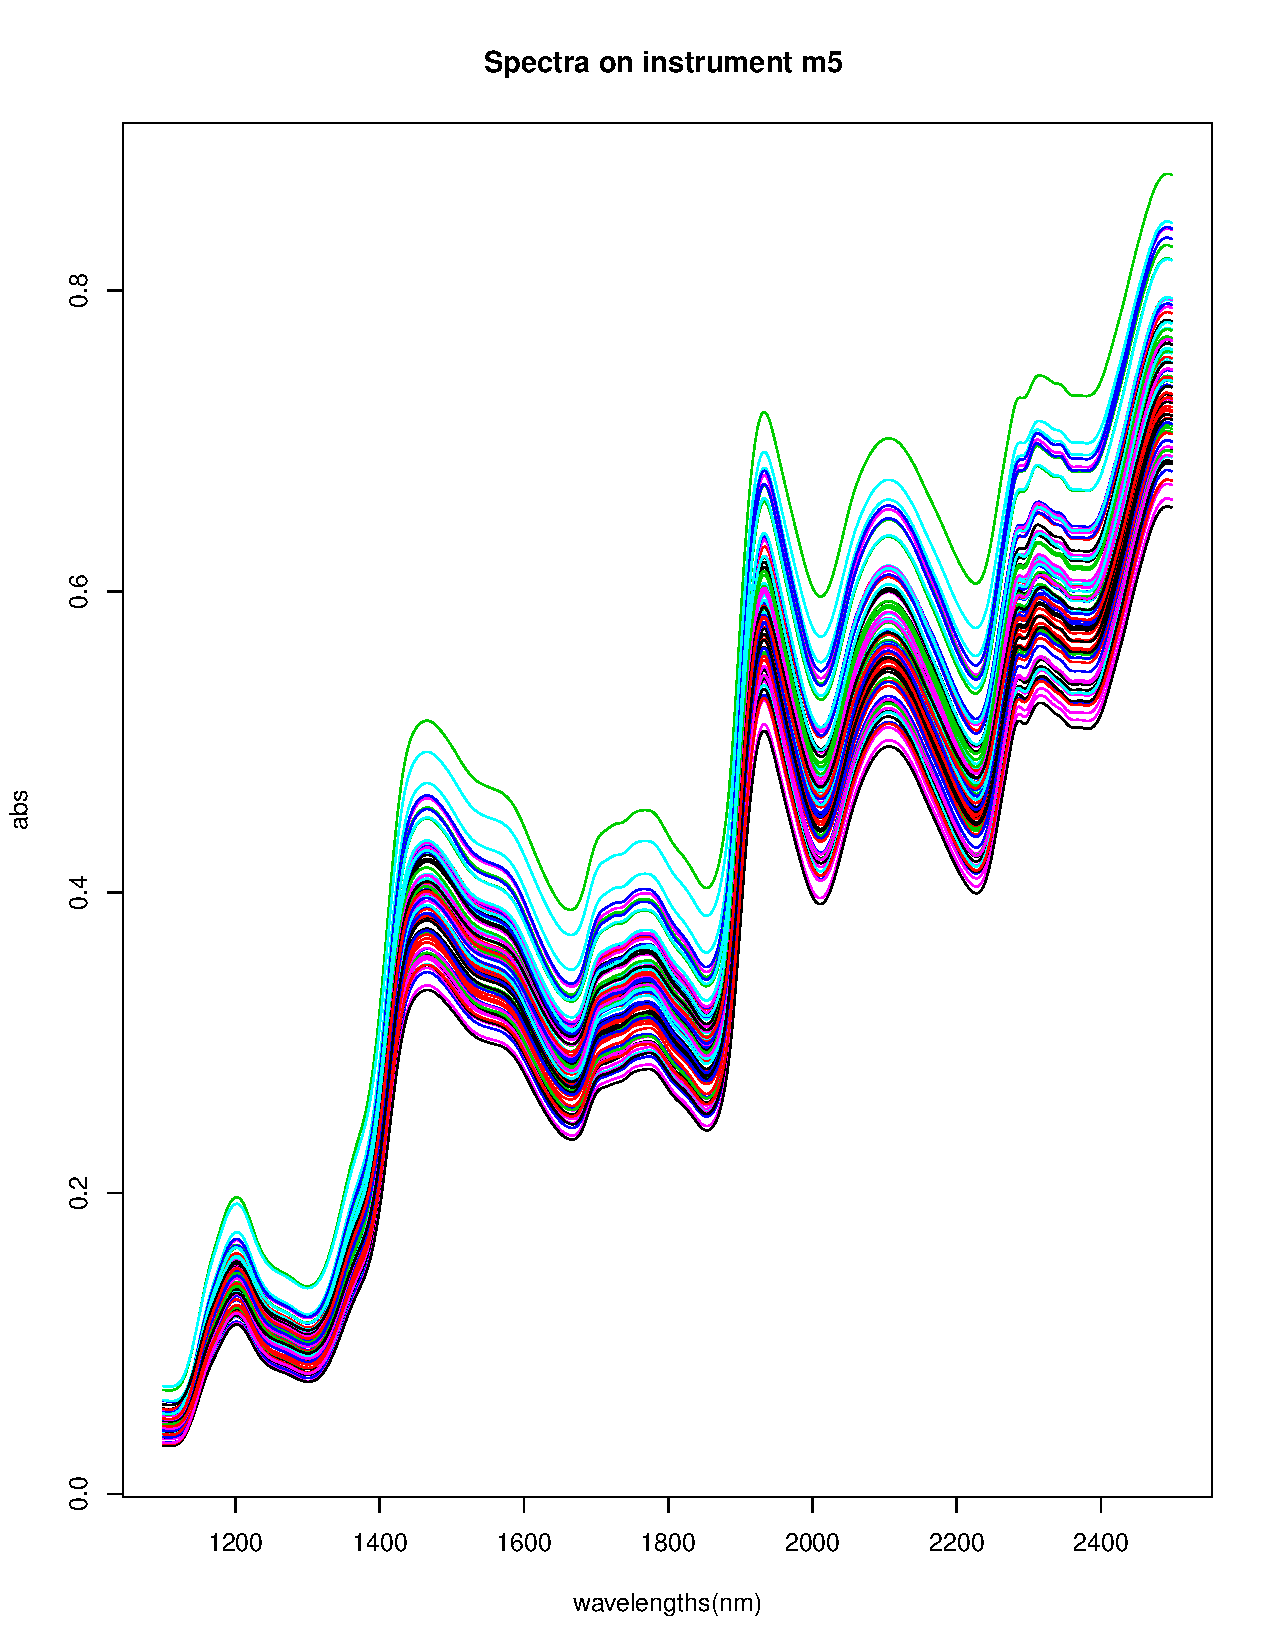
\includegraphics[width=7.5cm, angle=0]{Spectra_on_instrument_m5.pdf}  % width changes size
				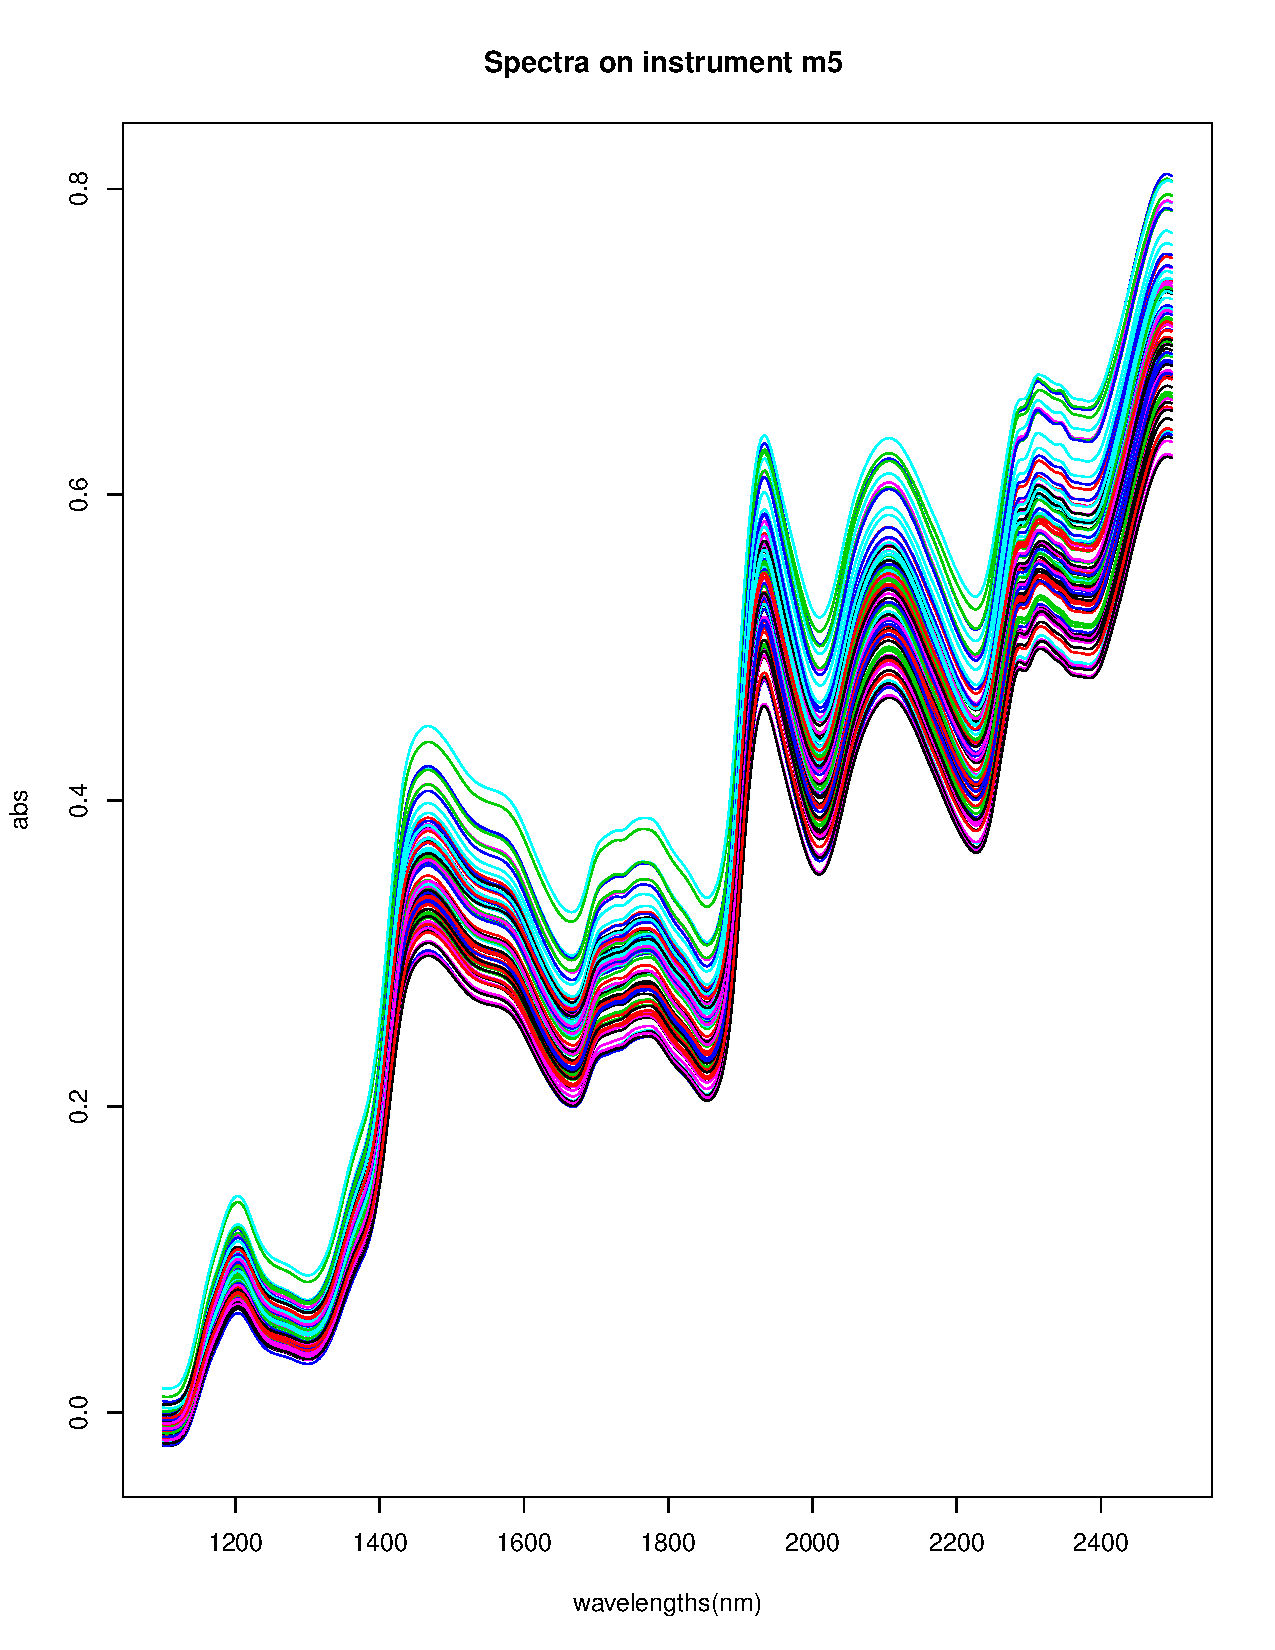
\includegraphics[width=7.5cm, angle=0]{Spectra_on_instrument_mp5.pdf}  % width changes size
		\caption{Spectra on instrument m5 and mp5}          % a meaningful caption
		\label{fig:Spectra_on_instrument_m5}               % label for the figure
	\end{figure}                        % end of figure environment
	
	 Each of these samples also gives the corresponding moisture, oil, protein and starch values. In this dissertation, the spectrum data measured by m5 spectrometers calls as m5. So the same as mp5 and mp6. And one of m5, mp5 and mp6 NIR data will be selected as $X$ in each regression. The value related to the moisture, oil, protein and starch values was considered as the dependent variable $Y$. So $X$ should be one of three 80$\times$700 matrices and $Y$ should be one of four 80$\times$1 vectors.
	  In addition, corn data set will be divided into a calibration set and a prediction set using a random sampling method. Model the calibration set and then predict prediction set. Finally, RMSECV and RMSEP are calculated as the criterion.
	
	Firstly, the effect of each conditions on partial least squares regression (PLSR) is observed by different performance of PLSR based on corn data under different conditions. Secondly find out as much papers using corn data as possible to compare the results in papers with the results in dissertation. In this way, we can observe whether the new algorithm has a significant improvement compared to PLSR. Finally, the F-test is used to test whether the new method is significantly different from PLS.
	
	

	
	\section{Methodology}
	\label{sec:method}
	
	\subsection{Model Evaluation}
	\label{sec:eva}
	According to the corn data literature, there are several measures that can be used to evaluate the performance of the model.

	1. Root Mean Square Error for Calibration samples (RMSEC) is proposed by \citet{2yun2014strategy}.
	
	2. RMSECV is mentioned by many papers \citep{8ji2015using}. And there are two cross-validation methods. One is leave one out cross-validation (LOOCV), mentioned by \citet{6zheng2015pretreating}. The other is K-fold cross-validation, there are the 3-fold cross-validation \citep{3galvao2007cross}, 10-fold cross-validation \citep{8ji2015using} and so on. The calculation method of RMSECV is as follows:
	
	\begin{equation}
	RMSECV=\sqrt{\frac{1}{n}\sum_{i=1}^{n} (y_i-\hat y_i)^2} 
	\end{equation}
	\begin{conditions}
		n     &  the number of samples\\
		y_i     &   the experimental value of the i-th sample\\   
		\hat y_i &  the predicted value of the i-th sample by cross-validation which  includes removing the set of i-th sample from the calibration set, building a model with the remaining samples, and applying the model to i-th sample
	\end{conditions}
	
	3. The Root Mean Square Error of Prediction (RMSEP) is mentioned by \citet{1su2006partial}. This is a generally accepted method of evaluating models. This approach requires the determination of appropriate cross-validation sets and prediction sets before building PLS model. For example, 60 samples of corn data are used for a cross-validation and the remaining 20 samples are used as predictions \citep{1su2006partial}. Then the cross-validation data is used for modelling, determining the parameters for regression model, such as PLS. After that, the model is applied to the predictive data to calculate the Root Mean Square Error of Prediction (RMSEP). The RMSEP calculation formula is:
	
	\begin{equation}
	RMSEP=\sqrt{\frac{1}{m}\sum_{i=1}^{m} (y_i-\hat y_i)^2}
	\end{equation}
	
	\begin{conditions}
		m     &  the number of prediction sets\\
		y_i     &  the experimental value of the i-th sample in the prediction set \\   
		\hat y_i &  the prediction value of model for the i-th sample
	\end{conditions}
	
	
	4. There are few papers mentioned that $R^2$ is used to measure the model \citep{tatavarti2005assessment}. But this method is also flawed. In some situations, not enough calculation accuracy of the computer will cause the value of $R^2$ to be equal to 1. For example, \citet{deng2016bootstrapping} has this problem and the $R^2$ in PLS model fitting  moisture is equl to 0.9959, but for the CARS, GA-PLS and BOSS model, $R^2$ are all equal to $1.0000 \pm 0.0000$. Hence we can see it hard to distinguish the different between models. So this will not be a good indicator of evaluation.
	
	\subsection{Pre-treatment}
	\label{sec:treat}
	The papers use different pre-treatments of the data, and the results of the model will be very different. For example, \citet{7galvao2008variable} and \citet{8ji2015using} both use M5 to predict the first constituent, and the results are very different. Through the different literatures, the common pretreatment of corn data has the following four types:

	\begin{enumerate}
			
	\item Nothing to deal with \citep{1su2006partial}.
	
	\item Scale the data \citep{4ergon2006reduced}.
	
	\item SavitzkyGolay filter processing on the data \citep{3galvao2007cross}.
	
	\item Delete the outliers. For example \citet{8ji2015using} take out the 75th and 77th corn 
	spectrum from dataset as outliers.
	
	\end{enumerate}
	
	\subsection{Sample splitting}
	\label{splitting}
	The number of samples selected and the method of sample selection will also have an impact on the results of models. The methods of selecting samples are as follows:
	
	\begin{enumerate}
	
	\item A completely random sample \citep{1su2006partial}.
	
	\item Choosing the samples by SPXY method \citep{3galvao2007cross}.
	
	\item Use the Kennard-Stone (K-S) algorithm \citep{zhao2015optimization}.
	
	\item Directly divide the raw data into the first half and the second half, the first half is cross-validation sets, and the second half is prediction set \citep{4ergon2006reduced}.

	\end{enumerate}
	
	The second and third methods will result in the prediction level data being very close to the data of the cross-validation set, which may increase the accuracy of the prediction and reduce the prediction difficulty, so these two methods are not used here. Because in the actual problem, the performance of the algorithm looks better when the two sample sets are too similar, which is not what we want. The last method relies on the sorting of the original data, so the next step is to take a random sampling method to simulate the sample. The selection of samples refers to \citet{5zheng2012stability} and \citet{6zheng2015pretreating}, so the sample size of 20 $\sim$ 70 will be selected as calibration to build the model, and the rest will selected as prediction.
	
	\subsection{Cross-validation}
	\label{cross-validation}
	The cross-validation is to divide the data into n groups. One of group is selected as the prediction set, and the remaining n-1 groups are used as calibration sets, and testing n times. Finally, the average of results of all tests was taken as the cross-validation result. If the selected n is the same as the size of sample, then this method is called leave one out method (LOO), otherwise it is called the k-fold cross-validation. Cross-validation not only improves the reliability of models, but also allows the model to avoid falling into local optimal solutions. Figure \ref{fig:cross-validation} shows the flow of the cross-validation.
	\begin{figure}[h]    % start of figure environment
		\centering           % put the graph(s) in the centre of the page (horizontally)
		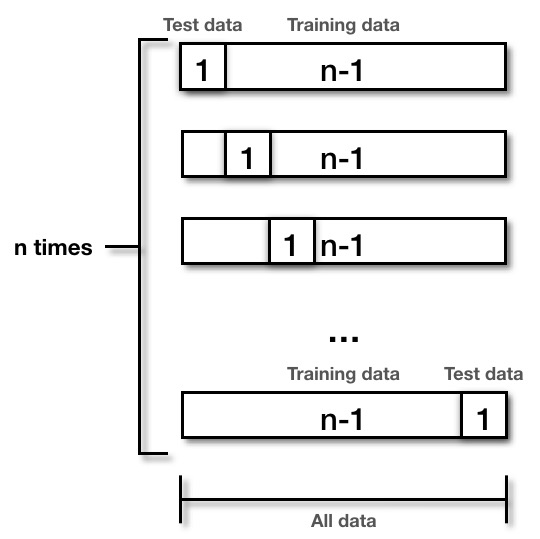
\includegraphics[width=8.5cm, angle=0]{cross-validation.png}  % width changes size
		\vspace*{-0.25cm}    % manual adjustment of vertical spacing
		\caption{The flow of the cross-validation}          % a meaningful caption
		\label{fig:cross-validation}               % label for the figure
	\end{figure}                        % end of figure environment
	
	The choice between LOO and k-fold cross-validation is determined according to the number of samples. When the sample size is small, the LOO is preferred. When the sample size is too large, the k-fold cross-test is preferred. There is an additional reminder here that the difference between LOO and the k-fold cross-validation is not just a difference in computing time. More, when the sample size is too large, LOO may cause over-fitting problems, and the k-fold cross-validation can not only save computational power, but also avoid the over-fitting problem in here. Chapter \ref{sec:Cross-Validation} will discuss the difference.
	
	\subsection{PLS algorithm}
	\label{PLS_al}
	The partial least squares regression (PLS) is a multi-regression technique proposed by \citet{wold1984collinearity}, and it is also the most common statistical method in the research of near-infrared spectroscopy (NIR). Partial least squares regression is similar to principal components analysis (PCA) and is also a factor analysis method. In the modelling  process, it is first necessary to decompose the matrix of spectrum and then extract a few principal components (these variables are called latent variables in PLS) to represent most of the information of original spectrum. Because the spectral data is high-dimensional, the number of independent variables is more than the number of samples, thus it cannot meet the basic assumption of least squares method (OLS). Therefore, it is necessary to extracting the data to some components, and then make the regression. Compared with PCA, PLS not only considers the dimensionality reduction of the independent variables, but also maximizes the covariance between principal components and target variables. In this way, the covariance between the extracted components and the target vector will be the maximum. According to this point, PLS is the improvement and further development of PCA, and the results in many applications also prove that PLS has better performance than PCA.
	
	The process of partial least squares regression is as follows:
	
	The PLS model needs to perform principal component decomposition on the spectral data matrix and the target vector when it is established.
	
	\begin{equation}
	X=TP^T+E 
	\end{equation}
	\begin{equation}
	Y=UQ^T+F
	\end{equation}
	
	Where $T$ and $P$ are the score matrices and the loading matrices of the spectral matrix $X$, respectively. $U$ and $Q$ are the score matrices and the loading matrices of target vector $Y$. $E$ and $F$ are residual matrices of the spectral matrix $X$ and target vector $Y$, respectively, and $T$ and $U$ can perform linear regression as follows:
	
	\begin{equation}
	u_i=t_ib_i
	\label{equ:ui} 
	\end{equation}
	
	Here $t_i$ and $u_i$ are the first column data of $T$ and $U$, respectively.
	
	In the process of establishing partial least squares regression models, the spectral matrix $X$ and the target vector $Y$ are decomposed in an iterative manner. In each iteration, the principal components $t_i$ and $u_i$ of $T$ and $U$ can be obtained separately. Linear regression is performed on $t_i$ and $u_i$ by Equation (\ref{equ:ui}), and then the information explained by $t_i$ and $u_i$ is subtracted from spectral matrices and target vectors, respectively, to obtain the residual matrices. Finally, the residual matrices is brought into the previous iterative process again, which are the spectral matrices and the target vectors in next iteration. This iterative process is terminated by constant iteration until the latent variable of the specified target is obtained. The specific operation flow, pseudocode as follows:
	
	\begin{enumerate}
	
	\item Initialize the score vector $u=Y$.
	
	\item Calculate the weight vector $\omega$ by formula \ref{equ:omega}:
	
	\begin{equation}
	\omega=X'u/(u'u)
	\label{equ:omega} 
	\end{equation}
	
	\item Let $\omega=\omega/\left\|\omega\right\|$.
	
	\item Calculate the spectral score vector $t=X\omega$.
	
	\item Calculate the spectral matrices' loading vector $p=X't/(t't)$.
	
	\item According to the spectral matrix score vector, calculate target vector $q=Y't(t't)$.
	
	\item Let $X=X-tp'$ and $Y=Y-tq$.
	
	\item If the number of extracted latent variables reaches number required by the algorithm, the iteration is terminated, otherwise go back to step 1 and continue the next iteration.
	
	\end{enumerate}
	
	After the iteration process finish, the regression coefficients of the partial least squares regression model (PLSR) are calculated according to the equation \ref{equ:B}.
	\begin{equation}
	B=W(P'W)^{-1}Q
	\label{equ:B} 
	\end{equation}
	
	Finally, the prediction model of the partial least squares regression model is as equation \ref{equ:y_unknow}.
	\begin{equation}
	Y_{unknow}=X_{unknow}B
	\label{equ:y_unknow} 
	\end{equation}
	
	\subsection{Parallel computing}
	\label{parallel}
	
	Parallel computing is the simultaneous calculation of tasks that are broken down into subtasks into multiple cores. There are two computer calculation ways: serial calculations, such as iterative algorithms, and parallel calculations, such as repeated experiments. When an algorithm calculations are all serial tasks, it is completely impossible to use parallel computing. When all the calculations from an algorithm are parallel tasks, then full parallel computing can be used. So, how much parallel computing can improve algorithm, it depends on the proportion of the algorithm's serial computing part and parallel computing part respectively. When there are less serial calculations in algorithm, the more time can be saved by parallel computing. In this dissertation, each partial least square regression process is a serial calculation and cannot be optimized by  parallel computing. However, repeated experiments with partial least squares regression can be optimized using parallel computing.
	
	Because this dissertation is computationally heavy, parallel computing is considered to improve the efficiency of algorithm. Through the analysis of a small amount of experimental data, it is estimated that if a single-core calculation is used, the computation required to complete the whole paper will take about three months to end the calculation. In terms of time, if  dissertation doesn't optimize the algorithm, this is an impossible task to finish dissertation in time.
	
	Parallel computing in R language is divided into two categories, one is implicit parallel computing and the other is explicit parallel computing. Implicit parallel computing hides most of the parallel computing details from the user, and the user does not need to know the specific calculation process. After library the implicit parallel computing related R packages, the system automatically enables parallel computing based on the current resources. The related R package includes "OpenBLAS", "Intel MKL" and "NVIDIA cuBLAS". But the disadvantage of this kind of parallel computing is that the efficiency of the upgrade is extremely limited. The other is explicit parallel computing. Explicit parallel computing requires the user to actively run parallel computing, and actively divide the data and assign tasks. This type of parallel computing can effectively improve the efficiency of the algorithm, but not as friendly as the former. The associated R language explicit parallel package includes "parallel", "foreach", "SupR" and "gpuR". Whether it is implicit parallel computing or parallel computing, parallel computing consumes a lot of memory, and the lazy evaluation programming strategy used by R exacerbates this problem. Therefore, when using parallel computing, you need to allocate enough memory space in advance to the program. This dissertation implements parallel computing through the family of "apply" functions optimized by "parallel" package in R.
	
	The main steps of complete parallel computing process are as follows:
	\begin{enumerate}
	\item  Load the parallel package and calculate the number of available cores. R code is as follows:
	\begin{lstlisting}[language=R]
	library(parallel) 
	clnum <- detectCores()
	\end{lstlisting}
	
	\item Initialize and set up a clustered parallel computing environment.
	
	\begin{lstlisting}[language=R]
	cl <- makeCluster(getOption("cl.cores", clnum))
	\end{lstlisting}
	
	\item Assign copies of packages and variables that need to be used in parallel computing to each core.
	
	\begin{lstlisting}[language=R]
	clusterExport(cl, "RawData")
	\end{lstlisting}
	
	\item Run the algorithm optimized for parallel computing.
Here is the optimized code sample as following:
	
	\begin{lstlisting}[language=R]
	Result <- parSapply(cl, x, my_function)
	\end{lstlisting}
	
	\item Shut down the cluster.
	
	
	\begin{lstlisting}[language=R]
	stopCluster(cl)
	\end{lstlisting}
	
	\end{enumerate}


	
	
	Enable different number of cores and running times as shown in Table \ref{parallel_time}. 
	
		\begin{table}[h]
		\centering
		\begin{tabular}{llllll}
			\hline
			Number of core & 1     & 9     & 18    & 27    & 36    \\ \hline
			Running time (s)  & 97.42 & 68.84 & 58.56 & 55.77 & 54.97 \\ \hline
		\end{tabular}
		\caption{Different number of cores vs. running time of parallel computing and one core means no parallel computing.}
		\label{parallel_time}
	\end{table}
	
	
	Table \ref{parallel_time} shows running time required for the corn data m5 spectrum to perform 5000 partial least squares regression on moisture data. As can be seen from the table, as the number of cores increases, the running time shows a significant downward trend. But when the number of cores exceeds a certain limit, the algorithm improvement through parallel computing is getting smaller and smaller. This is because, when the number of cores is too large, it will take a lot of time to allocate subtasks to the initialization process of each core. But when the amount of calculation becomes larger, parallel computing will show its superiority.
	

	

	
	\subsection{High performance computing (HPC)}
	\label{myriad}
	
	High-performance computers are also often referred to as supercomputers. It is a cluster that is connected by a network of many servers called nodes. A cluster can simultaneously use multiple cores or multiple nodes to run multi-core tasks through a special network. And the reason why use high-performance computers for calculation in this dissertation is as follows.

	\begin{enumerate}
	\item Dissertation needs to run large parallel jobs. Usually, a single-core program needs to run continuously for 6$\sim$12 hours on personal computers every times. The personal computers cannot do anything  while running large parallel jobs, and you need to make sure computers do not encounter any unexpected situations, such as sleep, power outages, and accidental touches on the keyboard. So such a task is an unrealistic job to run locally.

	\item Dissertation needs large quantities of RAM. Because this thesis uses parallel computing so many times, it consumes a lot of computer memory than a single core compute. While personal computers usually have only 16 GB, less than half of the available memory can be allocated to programming. So in terms of memory requirements, personal computers are not good enough.

	\end{enumerate}

	This dissertation uses two high-performance computing systems ,named "Myriad" and "Grace", provided by University College London. "Grace" consists of 684 compute nodes, 10,944 processor cores and over 1 Petabyte high-performance memory, which is the largest and fastest high-performance computing system in the UK university sector.  And there are two ways to run r code through a cluster.

	\begin{enumerate}

	\item Load directly through commands in terminal and then use the R interactively. The codes for starting the R module are as follows.
	
	
	\begin{lstlisting}[language=sh]
	module unload compilers mpi
	module load r/recommended
	R
	\end{lstlisting}
	
	After setting anaconda environment, the interactive operation interface under tmux shell is as Figure \ref{fig:R_cluster}.
	
	\begin{figure}[h]    % start of figure environment
	\centering           % put the graph(s) in the centre of the page (horizontally)
	\includegraphics[width=14.5cm, angle=0]{"R_cluster".jpeg} % angle changes orientation
	\vspace*{-0.25cm}    % manual adjustment of vertical spacing
	\caption{R interactive operation interface under tmux shell}          % a meaningful caption
	\label{fig:R_cluster}               % label for the figure
	\end{figure}                        % end of figure environment
	
	
	\item Submit the task to the cluster through a batch job. These functions can be implemented through a runscript. Among this R runscript, the following variables need to be set in script:  required max wallclock time, required max memory, and required number of cores when run. There are also other additional functions, such as output path, or sending a message to mailbox when the code finishes running. These functions can be implemented through scripts. Finally, enter the command, start R module, and run the specified R file.
	
	Simplified runscript is shown below.
	
	\begin{lstlisting}[language=sh]
#!/bin/bash -l
#$ -S /bin/bash                          #Set type of shell
#$ -pe mpi 36                            #Set number of cores
#$ -l tmpfs=30G                          #Set max memory
#$ -l h_rt=48:0:0                        #Set max wallclock time
#$ -wd /lustre/scratch/scratch/uczlhpe/output
                                         #Set working path
#$ -m eas                                #Set email notification
#$ -M xxx@ucl.ac.uk                      #Set email address

module unload compilers
module unload mpi
module load r/recommended
R CMD BATCH run.R                        #Run R code
	\end{lstlisting}
	
After completing the runscript, it can use "qsub" to submit this script into remote server queue and wait for it to run.
	
	\end{enumerate}
	
	Both methods have advantages and disadvantages.
	The first method requires online wait, but the submitted task can be run immediately, and is suitable for use in program testing or when running a single program. In the second method, although it takes a while to run the code, when running a large number of serial programs and large parallel programs, it is a more sensible choice to submit the script to the cluster for calculation. In contrast, the advantage of clustering can be found not only in a more stable and better configuration than PC. Using a cluster also allows you to run multiple files at once, and a cluster can have multiple nodes running on multiple files at the same time. By disassembling the computing tasks and submitting them to the cluster in batches, the single-core calculation that takes up to three months to complete can be completed in just one week.
	
	\section{Result and discussion}
	\label{sec:result}
	
	\subsection{Loop times}
	\label{sec:Loop times}
	
	Set different loop times and repeat PLSR to calculate how many loop times are needed to get stable results. Too small a number of cycles will result in very unstable results and large standard deviations. However, because of the limitations of computer, there are also upper limits on the number of loop times. If the program loops too many times, it will require a unimaginable long runtime.
	
	First, 40 samples were randomly selected as calibration set 40 samples as prediction set. Then make 10 as the number of component. Calculate the corresponding RMSECV and RMSEP. Then continue to cycle this process, get the figure of RMSECV and RMSEP based on different loop times. Through above steps, the  Figure \ref{fig:sd_RMSECV_RMSEP} based on the partial least squares result under different cycle times can be obtained. Left graph of Figure \ref{fig:sd_RMSECV_RMSEP} is RMSECV and the right boxplot is RMSEP.
	
	\begin{figure}[]    % start of figure environment
		\centering           % put the graph(s) in the centre of the page (horizontally)
		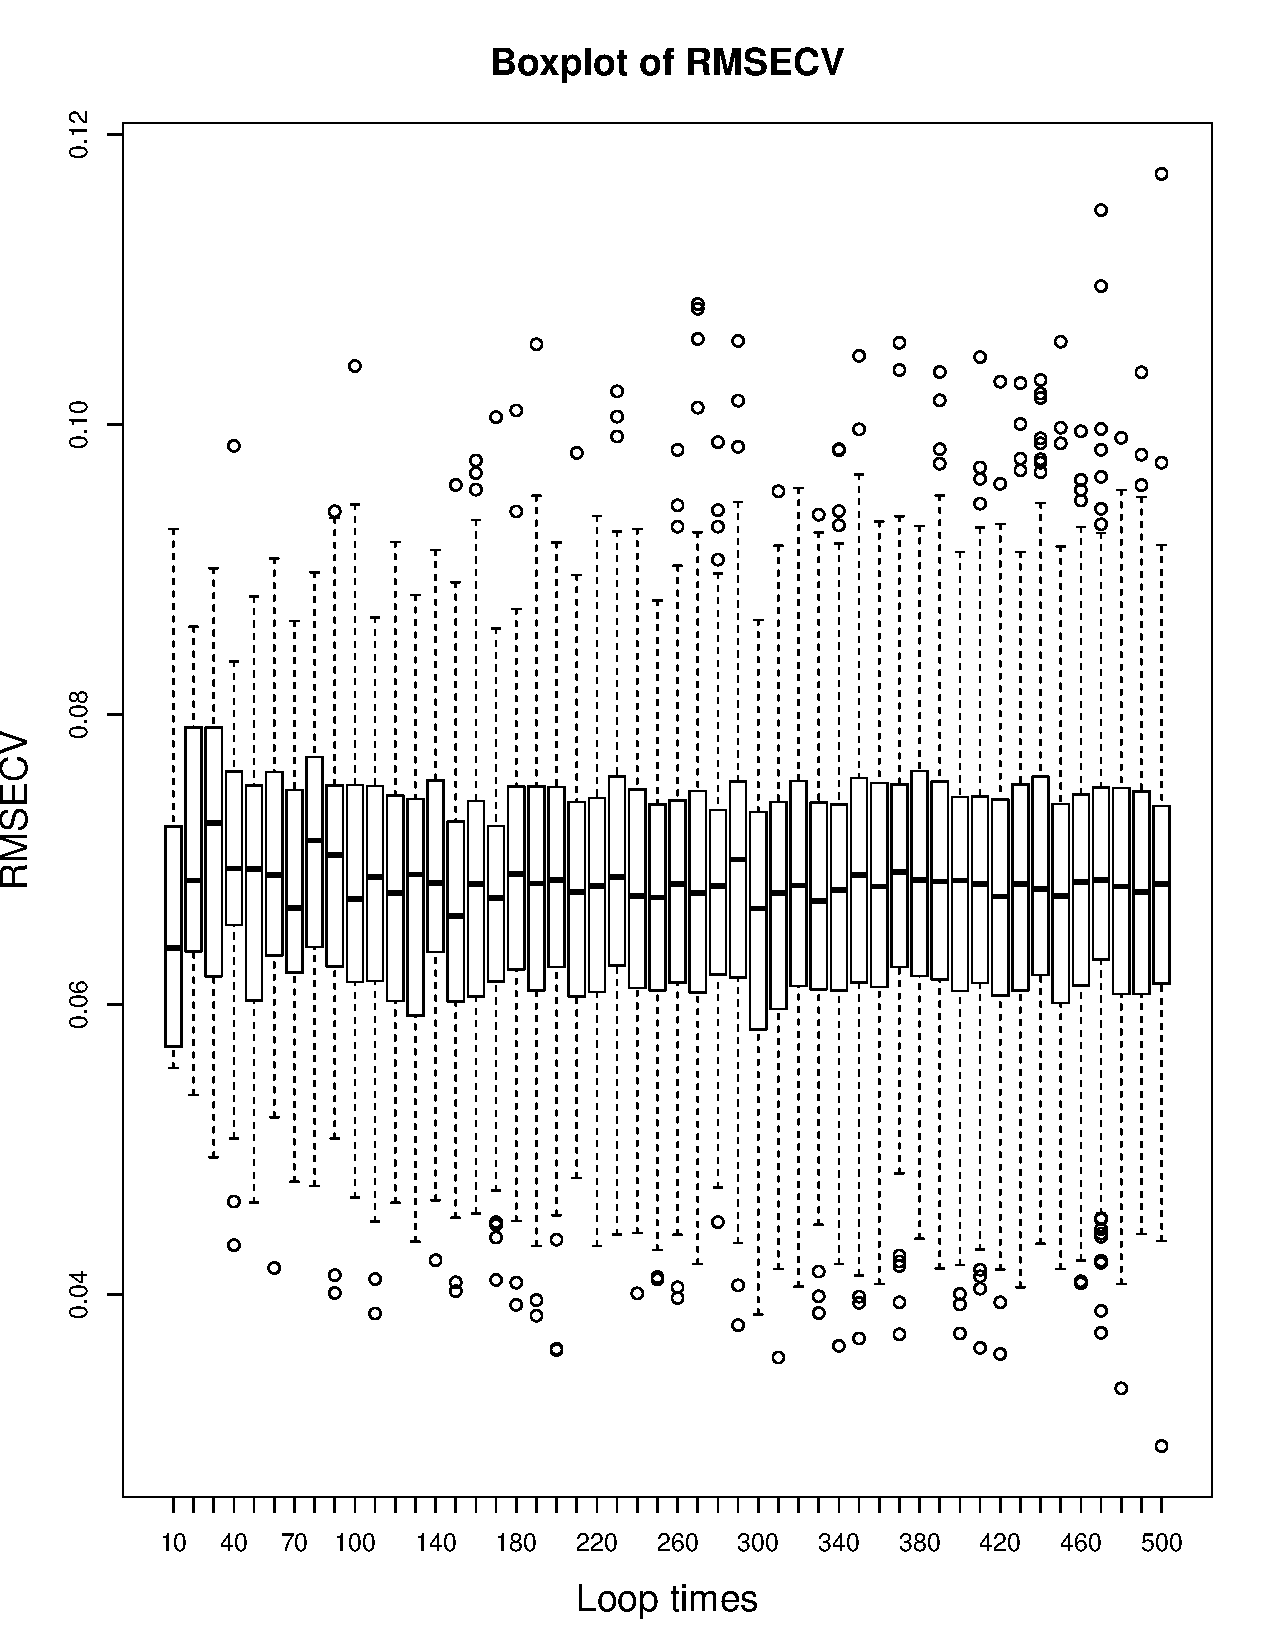
\includegraphics[width=5.5cm, angle=0]{boxplot_RMSECV_loop_times_500.pdf}  % width changes size
		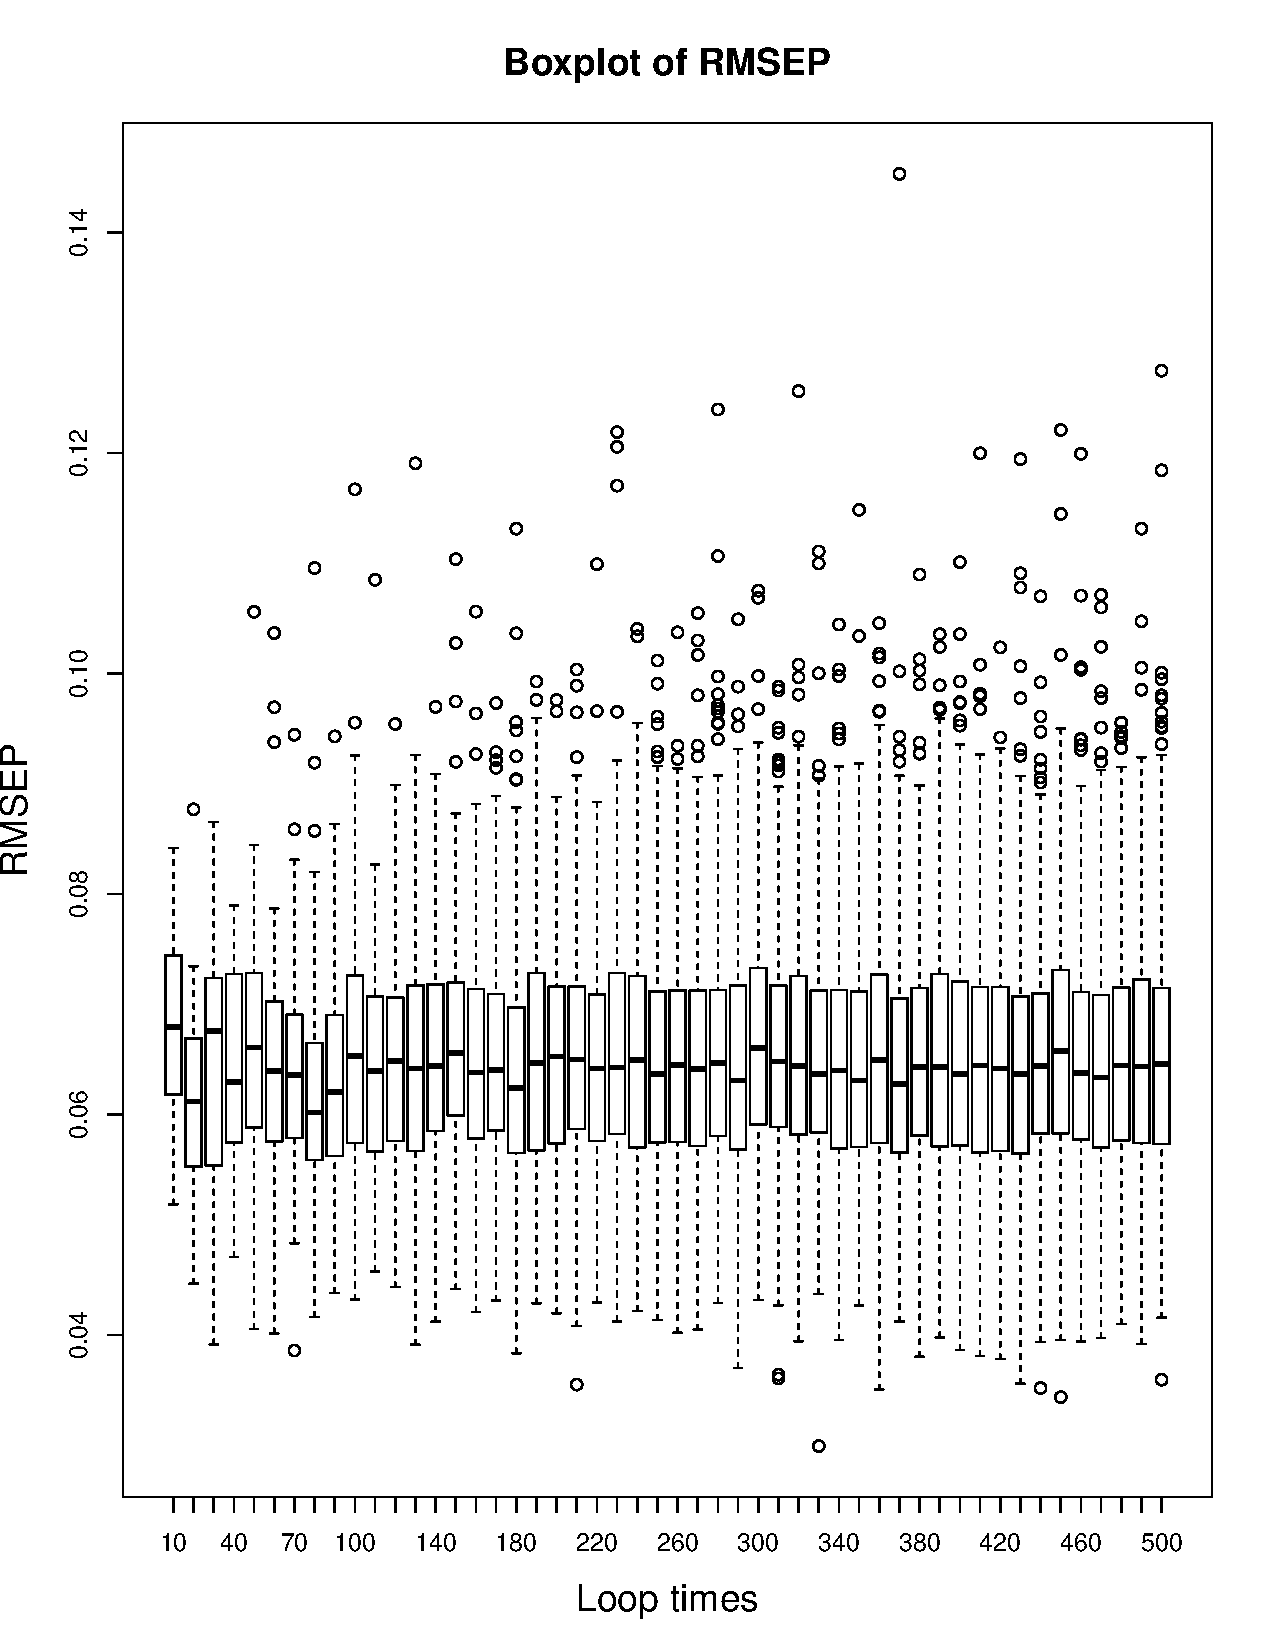
\includegraphics[width=5.5cm, angle=0]{boxplot_RMSEP_loop_times_500.pdf} % angle changes orientation
		%\vspace*{-0.25cm}    % manual adjustment of vertical spacing
		\caption{The boxplot of RMSECV and RMSEP from PLSR of oil on m5 under different loop times}          % a meaningful caption
		\label{fig:sd_RMSECV_RMSEP}               % label for the figure
	\end{figure}                        % end of figure environment
	
	
	 Figure \ref{fig:sd_RMSECV_RMSEP} shows that when the number of loops is too small, the results are not stable enough. When the number of cycles is less than 40, the result shows a significant deviation. But this table does not show how much the number of loops is appropriate. Therefore, the standard deviation plots based on loop times is made for before PLSR result. Figure \ref{fig:sd_RMSECV_loop_times_500} shows the standard deviations of RMSECV and RMSEP from PLSR of oil on m5 spectrum under different loop times.
	 
	 
	\begin{figure}[]    % start of figure environment
		\centering           % put the graph(s) in the centre of the page (horizontally)
		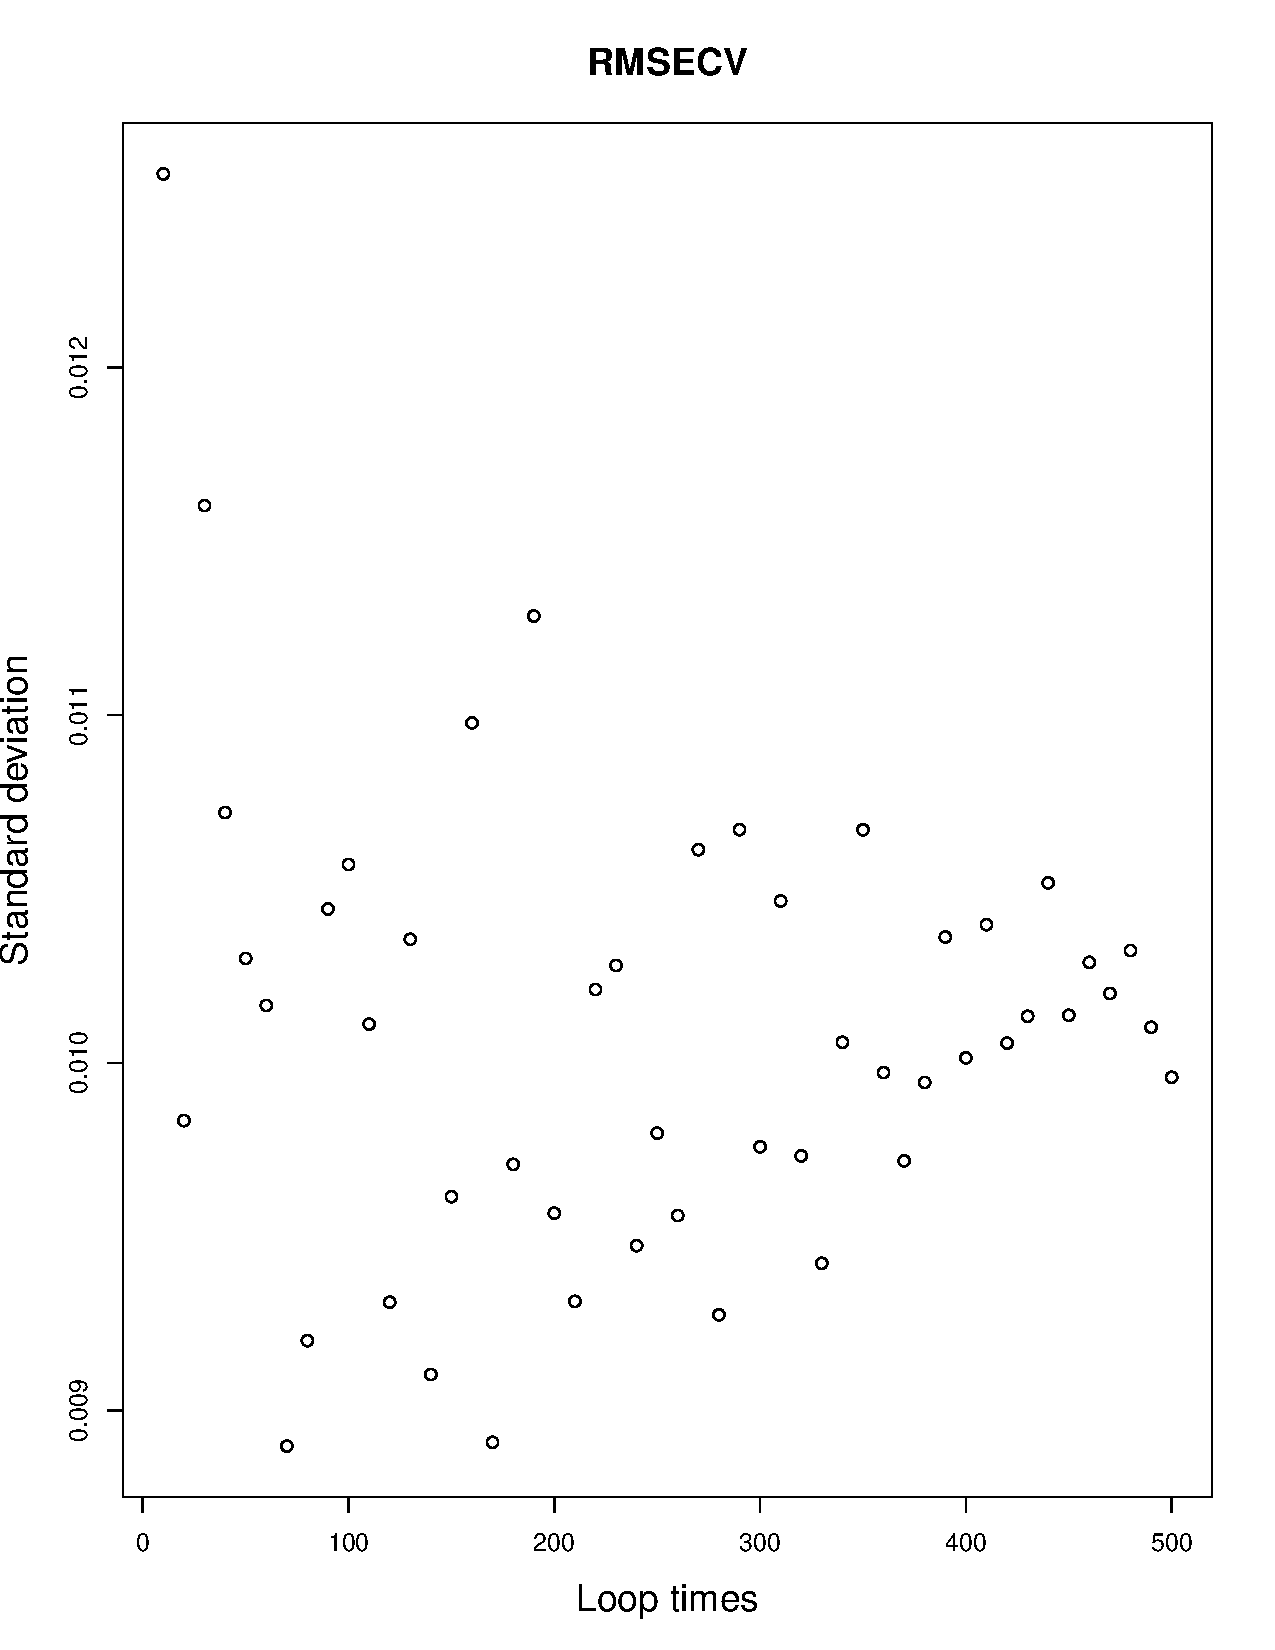
\includegraphics[width=5.5cm, angle=0]{sd_RMSECV_loop_times_500.pdf}  % width changes size
		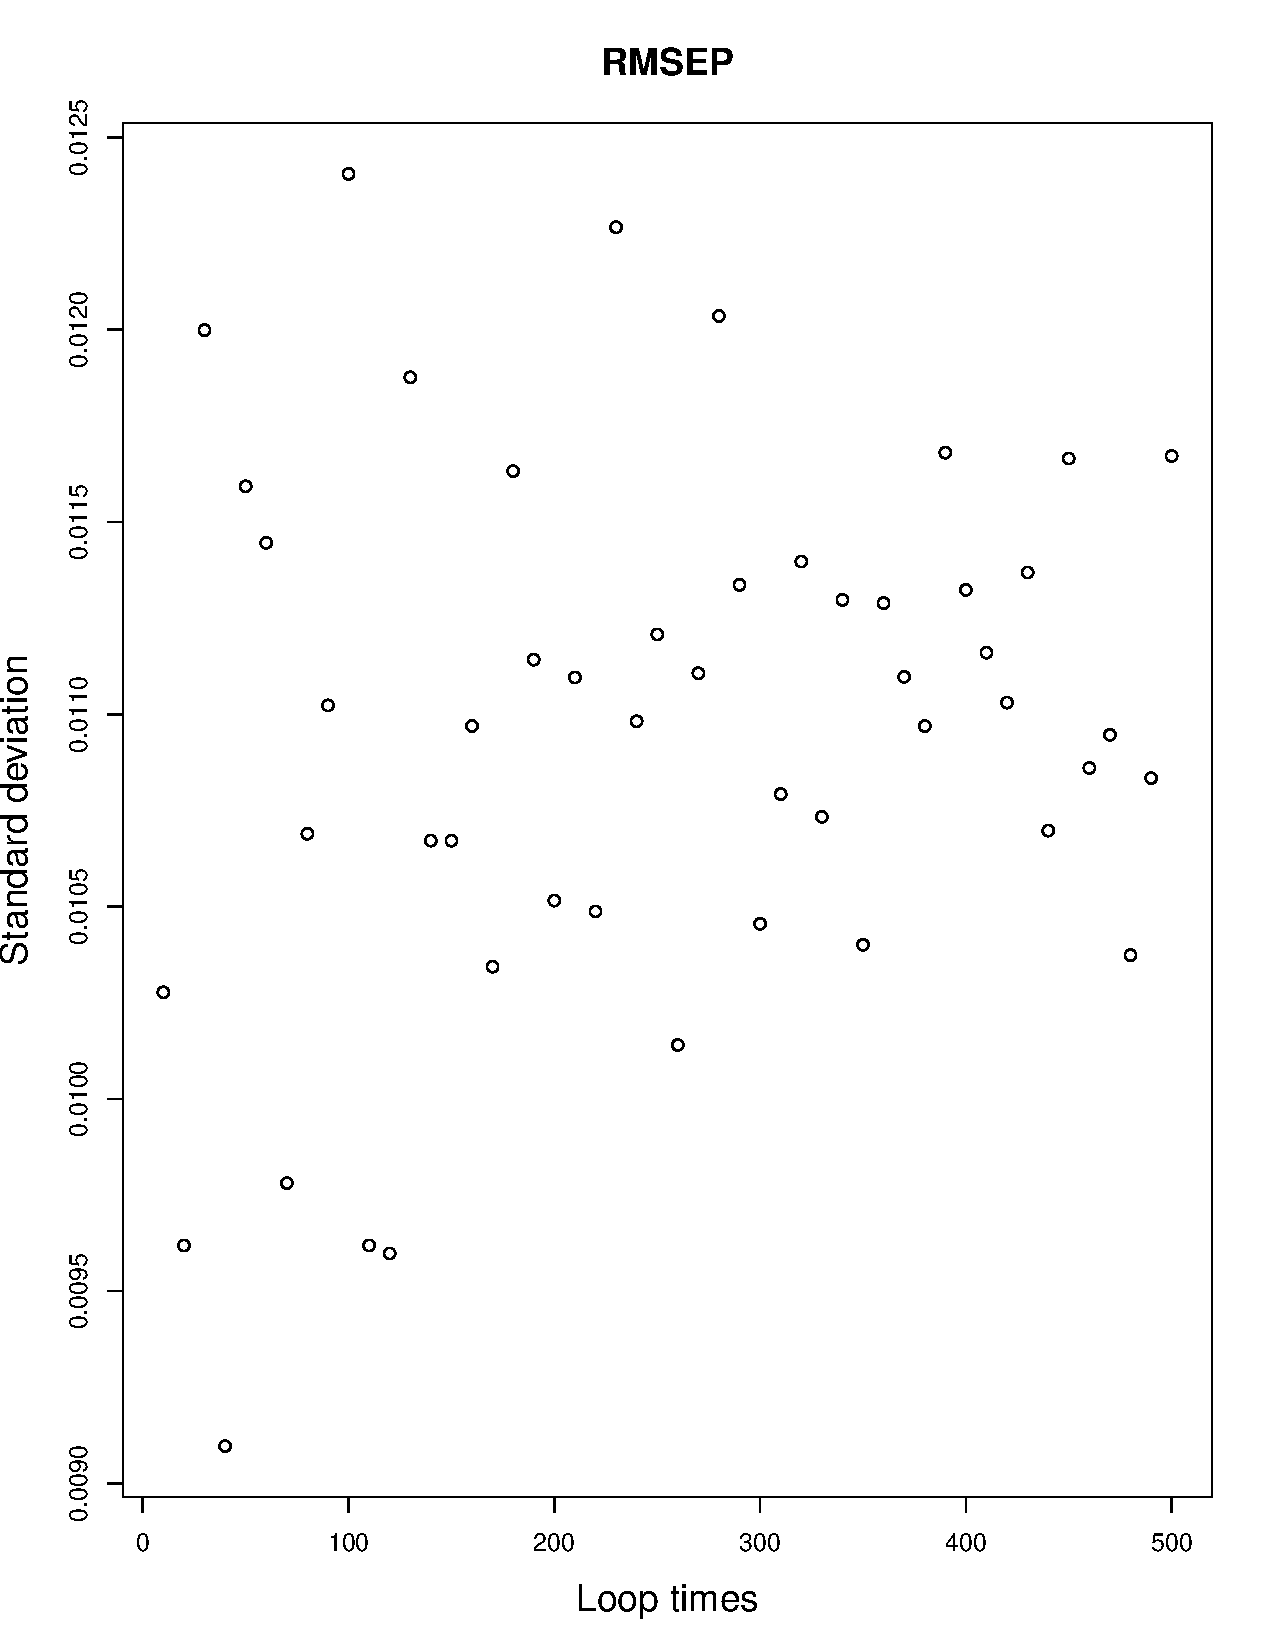
\includegraphics[width=5.5cm, angle=0]{sd_RMSEP_loop_times_500.pdf} % angle changes orientation
		%\vspace*{-0.25cm}    % manual adjustment of vertical spacing
		\caption{The standard deviation of RMSECV and RMSEP from PLSR of oil on m5 under different loop times}          % a meaningful caption
		\label{fig:sd_RMSECV_loop_times_500}               % label for the figure
	\end{figure}                        % end of figure environment
	
	
	Figure \ref{fig:sd_RMSECV_loop_times_500} shows that the standard deviations of RMSECV will decrease as the loop times increases. The RMSEP standard deviations will decrease with the increase of the loop times, and then tend to be stable. Through Figure \ref{fig:sd_RMSECV_loop_times_500} it is easy to see that the loop times is around 350, and the standard deviations of RMSEP will show the stable trends. Hence the number of loop times should be set 40$\sim$350 times to get a stable PLSR result. Because less than 40 the results will show a big fluctuation and there are not different results for the more than 350 loop times.
	
	\subsection{Number of samples}
	\label{sec:Number of Samples}
	
	Selecting different sample sizes as a calibration set has two different types of effects on PLSR. The difference between the two different types of effects is mainly in prediction part, the RMSEP. 
	
	The first effect is that as the number of sample in calibration set increases, the prediction of the model will become better and better. The RMSEP of PLSR will become smaller and smaller. When the number of sample in calibration set reaches a certain limit, the prediction of PLSR will tend to be stable. That is to say, regardless of the number of sample in calibration set, the RMSEP will tend to be stable. 
	
	Figure \ref{fig:samples_1} is the PLSR of moisture on m5 which is the first type effect. As the sample size increases, its prediction will stabilize.
	
				\begin{figure}[h]    % start of figure environment
		\centering           % put the graph(s) in the centre of the page (horizontally)
		\includegraphics[width=7.5cm, angle=0]{"/Users/hongwei/Documents/GitHub/STAT/MSc Project/paper_writing/number_of_calibration/unnamed-chunk-1-1".png}  % width changes size
		\includegraphics[width=7.5cm, angle=0]{"/Users/hongwei/Documents/GitHub/STAT/MSc Project/paper_writing/number_of_calibration/unnamed-chunk-1-2".png}  % width changes size
		%\vspace*{-0.25cm}    % manual adjustment of vertical spacing
		\caption{The RMSECV and RMSEP from PLSR of moisture on m5 under different number of calibration set.}          % a meaningful caption
		\label{fig:samples_1}               % label for the figure
	\end{figure}                        % end of figure environment
	
	The effect of the second type is that as the number of sample in calibration set increases, the RMSEP will drop significantly. As the sample size continues to increase to a threshold, the RMSEP will be very slowly smaller, but its variance will become larger and larger. In other words, the prediction of models will become more and more unstable. Please note that this is similar to the model's over-fitting, but it is not. The specific impact is that when the sample size is too big, each new sample will bring more but limited information to models, so the overall RMSEP will slowly decline. But when the calibration set size is much more than the prediction set, two things will happen. One is that the sample from calibration set will surround the predictors. This means that when using regression model for prediction, since there are enough calibration points similar to the prediction points, which makes the prediction easy, there may be cases where the RMSEP is extremely low. Another situation is that the calibration points do not surround the prediction points. The prediction point interval will not match the calibration point interval. This will lead to deviations in models. This makes RMSEP bigger. An extreme case can be considered when there is only one predicted point if the point is an outlier. Then the predictions will get very bad.
	
	As we can see Figure \ref{fig:sample_2}. The regression of the oil content on mp5 shows that this is second type effect. As the sample size increases, RMSEP will continue to decrease, but its variance will decrease first and then increase.
	
				\begin{figure}[h]    % start of figure environment
		\centering           % put the graph(s) in the centre of the page (horizontally)
		\includegraphics[width=7.5cm, angle=0]{"/Users/hongwei/Documents/GitHub/STAT/MSc Project/paper_writing/number_of_calibration/unnamed-chunk-6-1".png}  % width changes size
		\includegraphics[width=7.5cm, angle=0]{"/Users/hongwei/Documents/GitHub/STAT/MSc Project/paper_writing/number_of_calibration/unnamed-chunk-6-2".png}  % width changes size
		%\vspace*{-0.25cm}    % manual adjustment of vertical spacing
		\caption{The RMSECV and RMSEP from PLSR of oil on mp5 under different number of calibration set.}          % a meaningful caption
		\label{fig:sample_2}               % label for the figure
	\end{figure}                        % end of figure environment
	
	In order to research the specific impact of sample size on the PLS model. All corn data is used for regression.
	First select one of the three spectrums as an independent variable $X$. Then select one of the four constituents as the dependent variable $Y$. Set the number of components to 10. Use the leave-one-out cross validation and calculate the RMSECV of the model. Then the model is used to predict the remaining prediction samples. The predicted error deviation is recorded as RMSEP. Observe the changes in RMSECV and RMSEP by changing the number of calibration set samples. Finally, different independent variables $X$ from three spectrums and different dependent variables $Y$ from four constituents are selected to continue the PLSR. The specific calculation results of the complete partial least squares model are detailed in Appendix \ref{app:Number_of_samples}.
	
	\subsection{Number of components}
	\label{sec:Number of Components}
	
	The number of components is the most important parameter in PLSR. A change in this parameter will result in a big change in PLSR. The number of components represents that several independent variables will be selected as regressions in PLSR. As the number of components increases, the regression performe of models should be getting better and better. However, when the number of components is too large and over the threshold, there will be a situation of overfitting. The model's RMSECV and RMSEP will be reduced to a minimum and then rise again, and the variance will gradually increase during the rise process.
	
	The Figure \ref{fig:component_1} shows that the PLSR of starch content on mp5 under different number of components. From the Figure \ref{fig:component_1} we can see that when the number of components exceeds 10, RMSECV and RMSEP will become larger and more unstable.
	
		\begin{figure}[h]    % start of figure environment
		\centering           % put the graph(s) in the centre of the page (horizontally)
		\includegraphics[width=7.5cm, angle=0]{"/Users/hongwei/Documents/GitHub/STAT/MSc Project/paper_writing/number_of_components/unnamed-chunk-8-1".png}  % width changes size
		\includegraphics[width=7.5cm, angle=0]{"/Users/hongwei/Documents/GitHub/STAT/MSc Project/paper_writing/number_of_components/unnamed-chunk-8-2".png}  % width changes size
		%\vspace*{-0.25cm}    % manual adjustment of vertical spacing
		\caption{The RMSECV and RMSEP from PLSR of starch on mp5 under different number of components. And 60 samples as calibration set take leave-one-out as cross validation.}          % a meaningful caption
		\label{fig:component_1}               % label for the figure
	\end{figure}                        % end of figure environment
	
	The reason for the deterioration of the regression model is that too many principal components include some irrelevant details as part of the model, so the prediction set will be poorly predicted. This is the significant over-fitting problem we often say.
	
	All the regression results on different components show in Appendix \ref{app:Number_of_components}.
	It is worth noting that when the independent variable $X$ selects the m5 spectrum, Figures \ref{fig:components_1-1}, \ref{fig:components_2-1}, \ref{fig:components_3-1}, \ref{fig:components_4-1} show a trend that violates theory. As the number of components selected increases, the RMSECV and RMSEP  will continue to decrease and eventually stabilize. The reasons for this trend are not yet explained. So in the future this can be used as a research direction.
	
	\subsection{Pre-treatment}
	\label{sec:Pre-treatment}
	
	In section \ref{sec:treat}, there were four common pretreatments. The last pre-processing is to delete the outliers. When the outliers are deleted, the model can be unaffected by extreme values, so that a better model can be established. However, the subjectivity of this scheme is too strong, so quantitative discussions cannot be conducted here. So this dissertation focuses on three different treatments.
	\begin{enumerate}
	\item Nothing to deal with data \citep{1su2006partial}.
	
	\item Scale the data \citep{4ergon2006reduced}.
	
	\item SavitzkyGolay filter processing on the data \citep{3galvao2007cross}.
	
\end{enumerate}

First, the corn data was divided into two parts, among which 40 samples were randomly selected as the calibration set, and the remaining 40 samples were used as the prediction set. Then set the number of components to 10. Preprocess the data and then enter 100 cycles PLSR. The results of the calculations are available in Appendix \ref{app:pre-treatment}. The Figure \ref{fig:pre-treatment-1-1} is the boxplot of RMSECV and RMSEP from 100 loop times PLSR  of oil on m5 under different pre-treatment. "1" stands for none pre-treatment; "2" stands for scale $X$; "3" stands for savitzkyGolay filler with 1differentiation order, 2 polynomial order, 21 window size.
	
			\begin{figure}[h]    % start of figure environment
	\centering           % put the graph(s) in the centre of the page (horizontally)

	\includegraphics[width=7cm, angle=0]{"/Users/hongwei/Documents/GitHub/STAT/MSc Project/paper_writing/pre-treatment/unnamed-chunk-2-1".png}  % width changes size
	%\vspace*{-0.25cm}    % manual adjustment of vertical spacing
	\caption{The boxplot of RMSECV and RMSEP under different pre-treatment.}          % a meaningful caption
	\label{fig:pre-treatment-1-1}               % label for the figure
\end{figure}                        % end of figure environment
	
	As can be seen from Figure \ref{fig:pre-treatment-1-1}, standardization is the most inappropriate pre-processing of the data. According to all tables in Appendix \ref{app:pre-treatment}, it can be seen that the standardized pretreatment has the worst regression effect for each of the corn spectra.
	Because it has the largest rmsecv and rmsep. This is mainly because the standardization makes the value close to zero become close to "-1". Being close to zero in spectroscopy means that the spectrum at this band is meaningless. But standardization makes a number that was originally meaningless a non-zero value. This brings more useless information to the model. This is why standardization is a poor preprocessing method in spectroscopy.
	
	According to Appendix \ref{app:pre-treatment}, we can see that the regression results of the SavitzkyGolay filter are better than the results of no pre-treatment. This is mainly because SavitzkyGolay filter smoothes data, so that the data with the displacement can be corrected, and SavitzkyGolay filter preprocessing makes  regression models more robust. However, in some cases, no pre-processing will result in better results, so you need to consider the two before building the model.
	
	
	
	\subsection{Cross-validation}
	\label{sec:Cross-Validation}
	
	According to section \ref{cross-validation}, cross-validation is divided into two categories. In this dissertation will discuss leave-one-out cross-validation (LOO) and k-fold cross-validation (K-fold). The most intuitive difference is that LOO will consume more computer resources. But in fact, when the amount of data is too large, LOO will be more likely to fall into the over-fitting problem.
	
	In the process of regression modeling, cross-validation is the action that has the least impact on the results. However, if an inappropriate cross-validation is chosen, it will lead to overfitting or unstable regression results. Cross-validation will influence the process of selecting the number of components in PLSR. Figure \ref{fig:Cross-validation-1} is the RMSECV as a function of the number of components. The left image is based on LOO and the right image is based on 2-fold. It should be noted here that in order to unify the variable names in dissertation, the RMSECV here is the same variable as RMSEP in the cross-validation. 
	
		\begin{figure}[h]    % start of figure environment
		\centering           % put the graph(s) in the centre of the page (horizontally)
		\includegraphics[width=7.5cm, angle=0]{"LOO cross validation".pdf}  % width changes size
		\includegraphics[width=7.5cm, angle=0]{"K-fold cross validation".pdf}  % width changes size
		%\vspace*{-0.25cm}    % manual adjustment of vertical spacing
		\caption{RMSEP curves for the corn data under LOO cross-validation  and k-fold cross-validation.}          % a meaningful caption
		\label{fig:Cross-validation-1}               % label for the figure
	\end{figure}                        % end of figure environment
	
	Usually in the process of PLSR, we will select the corresponding number of components according to Figure \ref{fig:Cross-validation-1}. The inflection point and the lowest point are usually chosen. In Figure \ref{fig:Cross-validation-1}, according to the left side image, 11 will be the number of components under LOO, and according to 2-fold on the right side image, 9 will be the number of components. So, if using LOO, a larger number of components will be chosen. But Figure \ref{fig:Cross-validation-1} is not obvious, and because k-fold is random, we repeat the 2-fold as much as possible. The Figure \ref{fig:Cross-validation-2} shows the results based on 100 times 2-fold cross-validation. 
	
	
	
	
			\begin{figure}[h]    % start of figure environment
		\centering           % put the graph(s) in the centre of the page (horizontally)
		\includegraphics[width=7.5cm, angle=0]{"LOO cross validation2".pdf}  % width changes size
		\includegraphics[width=7.5cm, angle=0]{"K-fold cross validation2".pdf}  % width changes size
		%\vspace*{-0.25cm}    % manual adjustment of vertical spacing
		\caption{RMSEP curves for the corn data under LOO cross-validation  and k-fold cross-validation}          % a meaningful caption
		\label{fig:Cross-validation-2}               % label for the figure
	\end{figure}                        % end of figure environment
	
	Then zoom in Figure \ref{fig:Cross-validation-2} and fix the number of components from 7 to 18 to get Figure \ref{fig:Cross-validation-3}.
		
	\begin{figure}[h]    % start of figure environment
		\centering           % put the graph(s) in the centre of the page (horizontally)
		\includegraphics[width=7.5cm, angle=0]{"LOO cross validation3".pdf}  % width changes size
		\includegraphics[width=7.5cm, angle=0]{"K-fold cross validation3".pdf}  % width changes size
		%\vspace*{-0.25cm}    % manual adjustment of vertical spacing
		\caption{RMSEP curves for the corn data under LOO cross-validation  and k-fold cross-validation}          % a meaningful caption
		\label{fig:Cross-validation-3}               % label for the figure
	\end{figure}                        % end of figure environment
	
	As can be seen from the Figure \ref{fig:Cross-validation-3}, the RMSECV based on 2-fold is larger than the RMSECV based on LOO. This may cause RMSECV curve based on K-fold to enter the inflection point and the lowest point in advance. Thereby a smaller number of components is obtained. Moreover, the RMSECV based on LOO will be smaller than RMSECV based in K-fold at the same number of components. This is mainly because during the cross-validation process, LOO will use all data excepted one prediction sample to regress the one. At this time, the model will have better performance and will make the RMSECV value smaller, so when selecting the principal component, LOO will make people choose the bigger number of components.
	
	When the amount of sample data is small, the difference between LOO and K-fold is not obvious. However, it should be noted that when the amount of data is too large, the large number of principal components obtained from LOO can easily cause the model over-fitting, which is not what we hope. Unfortunately, the corn data sample is not large enough, so we can't clearly show the difference between LOO and K-fold here. finally, when the sample size looks like big, choosing cross-valiation should be carefully considered to prevent over-fitting problems.
	
	\subsection{Compare with papers}
	\label{sec:Compare with papers}
	
	The results of PLSR calculated in the previous were compared with the following eight papers. In most papers on corn data, PLSR is used as a reference algorithm. However, these PLSR results appearing in the paper only give RMSECV and RMSEP.  This has to question whether the new algorithm is really better than partial least squares regression, or the new algorithm is only one time that the regression result is better than PLSR.  Therefore, this dissertation uses the same parameters of PLSR as mentioned in other papers to repeat the experiments. The average and standard deviation of RMSECV and RMSEP were calculated by repeating 50 experiments every times. Then the calculated regression results are compared with the results of those papers.
	This dissertation compares with the following eight papers. Because the title of papers is too long, each paper is numbered for discussion. The results of the numbering are shown as following.
	
	\begin{enumerate}
		\item A Partial Least Squares‐Based Consensus Regression Method for the Analysis of Near‐Infrared Complex Spectral Data of Plant Samples \citep{1su2006partial}.
		
		\item A strategy that iteratively retains informative variables for selecting optimal variable subset in multivariate calibration \citep{2yun2014strategy}.
		
		\item Reduced PCR/PLSR models by subspace \citep{4ergon2006reduced}.
		
		\item Stability competitive adaptive reweighted sampling (SCARS) and its applications to multivariate calibration of NIR spectra \citep{5zheng2012stability}.
		
		\item Cross-validation for the selection of spectral variables using the successive projections algorithm \citep{3galvao2007cross}.   
		
		\item A variable elimination method to improve the parsimony of MLR models using the successive projections algorithm \citep{7galvao2008variable}.            
		
		\item Pretreating near infrared spectra with fractional order Savitzky–Golay differentiation (FOSGD) \citep{6zheng2015pretreating}.
		
		\item Using consensus interval partial least square in near infrared spectra analysis \citep{8ji2015using}
			
	\end{enumerate}
	
	As shown in Table \ref{tab:moisture}. The headers of the table mean:
	
	\begin{enumerate}
		
	\item Paper: the corresponding number can be found in section \ref{sec:Compare with papers} and each number corresponds to an identical paper.
	
	\item Data set: the regression models use one of m5, mp5 or mp6 spectrum as an independent variable $X$.
	
	\item Pre-treatment: preprocessing of corn data and SG(m,p,w) means m differentiation order, p polynomial order and w window size.
	
	\item Calibration set: the number of calibration set samples, and the corresponding number of prediction set samples is 80 - number of calibration set samples. The value in parentheses represent the type of cross validation.
	
	\item Number of components: the number of  components used in PLSR and it is the same as papers setting.
	
	\item Moisture: there are two sub-options of RMSECV and RMSEP under Moisture. All data representing this table is the regression of the moisture.
	
	\item PLS in papers: the PLSR result in corresponding numbered papers.
	
	\item Developed method: the new algorithm result from corresponding numbered papers.
	
\end{enumerate}
	
Table \ref{tab:moisture} is the PLSR result of moisture. Table \ref{tab:moisture} shows for the first paper, although the developed method has a smaller RMSEP compared to PLSR. However, the RMSEP of developed method in first paper is within one-fold variance of RMSEP by PLSR in this dissertation. So it's hard to think that the new method has a significant improvement over PLSR. The developed method in the second paper got a surprising RMSEP. This is a very surprising result and perhaps this is a fact. From this paper, we can't see anything obviously wrong, maybe it is true that selecting a small number of wavelengths works better for these data. In Table \ref{tab:moisture}, there are two lines of result for the third paper. The third paper claims that it uses the m5 spectrum, but in fact, according to the parameters mentioned in this paper, the mp5 spectrum is used to obtain the PLSR result which is more similar to the result in third paper. So the third paper might have used a different spectrum than it claimed. And according to the PLS result of the third paper, compared with the fourth paper. The PLS in third paper may use 10 components instead of the 12 it claims. But we can see from the results that its developed method has no better results than PLS. In the 4th, 5th 6th and 8th paper, according to the results in Table \ref{tab:moisture}, the developed method does have a better RMSEP than the PLS. It shows that these new methods have a better performance in the regression of moisture.

	Table \ref{tab:oil} is a regression result of the oil. According to Table \ref{tab:oil}, we can see that the developed method mentioned in the first paper is not very good, because the RMSEP based on developed method is similar to the RMSEP of PLSR. The new algorithm based on third paper has not seen a significant improvement compared to the PLSR. However, it is hard to judge whether there is not a significant difference between the new method and PLS. Also for the fifth paper, although the RMSEP based on the developed algorithm is smaller than the RMSEP based on PLSR, the difference between the new and old algorithm is small, and it is impossible to visually judge whether the developed algorithm and PLSR are significantly different. The seventh paper proposes a non-integral Savitzky–Golay differentiation method. The developed method has a more significant improvement than integral Savitzky–Golay filters with 0 and 1 differentiation order. But there is no way to tell that the new method has a significant difference compared to Savitzky–Golay filters with 2 differentiation order. And the new algorithm mentioned in the eighth paper also can not judge the obvious difference with PLS. 
	
	
	Table \ref{tab:protein} is a regression result of the protein. It can be seen from Table \ref{tab:protein} that the developed algorithm regression performance of the first and third paper is not much different from the PLSR. Even in some special cases, PLSR shows better regression results. The new regression model in the fifth, sixth and eighth paper has a significant improvement over the PLSR.
	
	
	Table \ref{tab:starch} is a regression result of the starch. Table \ref{tab:starch} shows that the results of the new algorithm in the first, third and seventh paper are not much different from those obtained from PLSR. The standard deviation of RMSEP can be used to measure the impact of random sampling on the results. From the standard deviation of RMSEP, it can be known that the PLSR has not a big probability that the new algorithm better than it. The new methods of the fifth, sixth and eighth papers all perform better than PLSR.
	
	\begin{landscape}
		
		%Table \ref{tab:moisture} is the regression for moisture.
		% Please add the following required packages to your document preamble:
		% \usepackage{multirow}
		\begin{table}[]
			\begin{tabular}{llllllllllllllll}
				\cline{1-13}
				\multicolumn{1}{c}{\multirow{2}{*}{Paper}} & \multicolumn{1}{c}{\multirow{2}{*}{\begin{tabular}[c]{@{}c@{}}Data\\ set\end{tabular}}} & \multicolumn{1}{c}{\multirow{2}{*}{\begin{tabular}[c]{@{}c@{}}Pre-\\ treatment\end{tabular}}} & \multirow{2}{*}{\begin{tabular}[c]{@{}l@{}}Calibration\\ set\end{tabular}} & \multirow{2}{*}{\begin{tabular}[c]{@{}l@{}}Number of\\ Components\end{tabular}} & \multicolumn{2}{c}{Moisture} &  & \multicolumn{2}{c}{PLS in papers} &  & \multicolumn{2}{c}{Developed method} &  &  &  \\ \cline{6-7} \cline{9-10} \cline{12-13}
				\multicolumn{1}{c}{} & \multicolumn{1}{c}{} & \multicolumn{1}{c}{} &            &    & RMSECV           & RMSEP           &   & RMSECV & RMSEP  &   & RMSECV  & RMSEP   &   &   &   \\ \cline{1-13}
				1                    & mp6                  & None                 & 60(LOO)    & 10 &                  & 0.148(0.0213)   &   &        & 0.159  &   &         & 0.139   &   &   &   \\
				2                    & m5                   & None                 & 64(5-fold) & 10 & 0.0152(0.000739) & 0.0202(0.00319) &   & 0.0149 & 0.0201 &   & 0.00026 & 0.00035 &   &   &   \\
				3                    & m5                   & Scale                & 40(LOO)    & 12 &                  & 0.0231(0.00443) &   &        & 0.3506 &   &         & 0.3485  &   &   &   \\
				3                    & mp5                  & Scale                & 40(LOO)    & 12 &                  & 0.159(0.0178)   &   &        & 0.3506 &   &         & 0.3485  &   &   &   \\
				4                    & mp5                  & Scale                & 40(LOO)    & 10 &                  & 0.405(0.0467)   &   &        & 0.357  &   &         & 0.265   &   &   &   \\
				5                    & m5                   & SG(1,2,13)*           & 60(3-fold) & 5  &                  & 0.0547(0.00942) &   &        & 0.040  &   &         & 0.012   &   &   &   \\
				6                    & m5                   & SG(1,2,21)*           & 60(LOO)    & 6  &                  & 0.0396(0.00625) &   &        & 0.045  &   &         & 0.019   &   &   &   \\
				8                    & m5                   & Delete 75 , 77       & 52(LOO)    & 10 & 0.0221(0.0018)   & 0.0194(0.00298) &   & 0.0124 & 0.0157 &   & 0.0047  & 0.0056  &   &   &   
			\end{tabular}
			
			\caption{regression of moisture.The values in parentheses corresponds to the cross-validation type in calibration set and standard deviation in moisture.
			*SG(m,p,w)=savitzkyGolay filler with m as differentiation order, p as polynomial order and w as window size.}
			\label{tab:moisture}
		\end{table}
		
		
		
		

		
		%Table \ref{tab:oil} is the regression for Oil.
		% Please add the following required packages to your document preamble:
		% \usepackage{multirow}
		\begin{table}[]
			
			\begin{tabular}{llllllllllllllll}
				\cline{1-13}
				\multicolumn{1}{c}{\multirow{2}{*}{Paper}} & \multicolumn{1}{c}{\multirow{2}{*}{\begin{tabular}[c]{@{}c@{}}Data\\ set\end{tabular}}} & \multicolumn{1}{c}{\multirow{2}{*}{\begin{tabular}[c]{@{}c@{}}Pre-\\ treatment\end{tabular}}} & \multirow{2}{*}{\begin{tabular}[c]{@{}l@{}}Calibration\\ set\end{tabular}} & \multirow{2}{*}{\begin{tabular}[c]{@{}l@{}}Number of\\ Components\end{tabular}} & \multicolumn{2}{c}{Oil} &  & \multicolumn{2}{c}{PLS in papers} &  & \multicolumn{2}{c}{Developed method} &  &  &  \\ \cline{6-7} \cline{9-10} \cline{12-13}
				\multicolumn{1}{c}{} & \multicolumn{1}{c}{} & \multicolumn{1}{c}{} &            &    & RMSECV          & RMSEP           &   & RMSECV & RMSEP  &   & RMSECV & RMSEP          &         &    &                 \\ \cline{1-13}
				1                    & mp6                  & None                 & 60(LOO)    & 10 &                 & 0.0991(0.0161)  &   &        & 0.107  &   &        & 0.0948         &         &    &                 \\
				3                    & m5                   & Scale                & 40(LOO)    & 14 &                 & 0.396(0.0665)   &   &        & 0.6912 &   &        & 0.6902         &         &    &                 \\
				3                    & mp5                  & Scale                & 40(LOO)    & 14 &                 & 0.694(0.095)    &   &        & 0.6912 &   &        & 0.6902         &         &    &                 \\
				5                    & m5                   & SG(1,2,13)*           & 60(3-fold) & 12 &                 & 0.0329(0.00672) &   &        & 0.029  &   &        & 0.022          &         &    &                 \\
				6                    & m5                   & SG(1,2,21)*           & 60(LOO)    & 10 &                 & 0.0505(0.0103)  &   &        & 0.028  &   &        & 0.030          &         &    &                 \\
				7                    & m5                   & SG(0,2,13)*           & 64(5-fold) & 7  & 0.0827(0.00419) & 0.0716(0.0116)  &   & 0.0729 & 0.0855 &   &        & 0.0400         &         &    &                 \\
				7                    & m5                   & SG(1,2,13)*           & 64(5-fold) & 7  & 0.0639(0.00357) & 0.0548(0.012)   &   & 0.0577 & 0.0682 &   & 0.0363 & 0.0400         &         &    &                 \\
				7                    & m5                   & SG(2,2,13)*           & 64(5-fold) & 7  & 0.0480(0.00312) & 0.0368 (0.0088) &   & 0.0370 & 0.0397 &   & 0.0363 & 0.0400         &         &    &                 \\
				8                    & m5                   & Delete 75 , 77       & 52(LOO)    & 10 & 0.0651(0.00662) & 0.0604(0.00876) &   & 0.0613 & 0.0673 &   & 0.0483 & 0.0546         &         &    &                 
			\end{tabular}
			
			\caption{regression of oil. The values in parentheses corresponds to the cross-validation type in calibration set and standard deviation in moisture.
			*SG(m,p,w)=savitzkyGolay filler with m as differentiation order, p as polynomial order and w as window size.}
			\label{tab:oil}
		\end{table}

		%Table \ref{tab:protein} is the regression for protein.
		% Please add the following required packages to your document preamble:
		% \usepackage{multirow}
		\begin{table}[]
			\begin{tabular}{llllllllllllllll}
				\cline{1-13}
				\multicolumn{1}{c}{\multirow{2}{*}{Paper}} & \multicolumn{1}{c}{\multirow{2}{*}{\begin{tabular}[c]{@{}c@{}}Data\\ set\end{tabular}}} & \multicolumn{1}{c}{\multirow{2}{*}{\begin{tabular}[c]{@{}c@{}}Pre-\\ treatment\end{tabular}}} & \multirow{2}{*}{\begin{tabular}[c]{@{}l@{}}Calibration\\ set\end{tabular}} & \multirow{2}{*}{\begin{tabular}[c]{@{}l@{}}Number of\\ Components\end{tabular}} & \multicolumn{2}{c}{Protein} &  & \multicolumn{2}{c}{PLS in papers} &  & \multicolumn{2}{c}{Developed method} &  &  &  \\ \cline{6-7} \cline{9-10} \cline{12-13}
				\multicolumn{1}{c}{} & \multicolumn{1}{c}{} & \multicolumn{1}{c}{} &            &    & RMSECV           & RMSEP         &   & RMSECV & RMSEP  &   & RMSECV & RMSEP  &   &   &   \\ \cline{1-13}
				1                    & mp6                  & None                 & 60(LOO)    & 10 &                  & 0.141(0.0203) &   &        & 0.150  &   &        & 0.145  &   &   &   \\
				3                    & m5                   & Scale                & 40(LOO)    & 8  &                  & 0.349(0.051)  &   &        & 0.4466 &   &        & 0.4349 &   &   &   \\
				3                    & mp5                  & Scale                & 40(LOO)    & 8  &                  & 0.37(0.0485)  &   &        & 0.4466 &   &        & 0.4349 &   &   &   \\
				5                    & m5                   & SG(1,2,13)*           & 60(3-fold) & 6  &                  & 0.107(0.0195) &   &        & 0.119  &   &        & 0.040  &   &   &   \\
				6                    & m5                   & SG(1,2,21)*           & 60(LOO)    & 7  &                  & 0.102(0.0186) &   &        & 0.110  &   &        & 0.033  &   &   &   \\
				8                    & m5                   & Delete 75 , 77       & 52(LOO)    & 13 & 0.119 ( 0.0155 ) & 0.11(0.0169)  &   & 0.1080 & 0.1353 &   & 0.0429 & 0.0846 &   &   &   
			\end{tabular}
			
			\caption{regression of protein. The values in parentheses corresponds to the cross-validation type in calibration set and standard deviation in moisture.
			*SG(m,p,w)=savitzkyGolay filler with m as differentiation order, p as polynomial order and w as window size.}
			\label{tab:protein}
		\end{table}

		%Table \ref{tab:starch} is the regression for starch.
		% Please add the following required packages to your document preamble:
		% \usepackage{multirow}
		\begin{table}[]
			\begin{tabular}{llllllllllllllll}
				\cline{1-13}
				\multicolumn{1}{c}{\multirow{2}{*}{Paper}} & \multicolumn{1}{c}{\multirow{2}{*}{\begin{tabular}[c]{@{}c@{}}Data\\ set\end{tabular}}} & \multicolumn{1}{c}{\multirow{2}{*}{\begin{tabular}[c]{@{}c@{}}Pre-\\ treatment\end{tabular}}} & \multirow{2}{*}{\begin{tabular}[c]{@{}l@{}}Calibration\\ set\end{tabular}} & \multirow{2}{*}{\begin{tabular}[c]{@{}l@{}}Number of\\ Components\end{tabular}} & \multicolumn{2}{c}{Starch} &  & \multicolumn{2}{c}{PLS in papers} &  & \multicolumn{2}{c}{Developed method} &  &  &  \\ \cline{6-7} \cline{9-10} \cline{12-13}
				\multicolumn{1}{c}{} & \multicolumn{1}{c}{} & \multicolumn{1}{c}{} &            &    & RMSECV         & RMSEP         &   & RMSECV & RMSEP  &   & RMSECV & RMSEP          &         &    &               \\ \cline{1-13}
				1                    & mp6                  & None                 & 60(LOO)    & 10 &                & 0.35(0.056)   &   &        & 0.370  &   &        & 0.358          &         &    &               \\
				3                    & m5                   & Scale                & 40(LOO)    & 9  &                & 0.393(0.0736) &   &        & 0.5010 &   &        & 0.4443         &         &    &               \\
				3                    & mp5                  & Scale                & 40(LOO)    & 9  &                & 0.513(0.0779) &   &        & 0.5010 &   &        & 0.4443         &         &    &               \\
				5                    & m5                   & SG(1,2,13)*           & 60(3-fold) & 6  &                & 0.239(0.0449) &   &        & 0.196  &   &        & 0.100          &         &    &               \\
				6                    & m5                   & SG(1,2,21)*           & 60(LOO)    & 5  &                & 0.258(0.0453) &   &        & 0.228  &   &        & 0.101          &         &    &               \\
				7                    & m5                   & SG(0,2,13)*           & 64(5-fold) & 8  & 0.333(0.0226)  & 0.283(0.0624) &   & 0.312  & 0.214  &   & 0.240  & 0.219          &         &    &               \\
				7                    & m5                   & SG(1,2,13)*           & 64(5-fold) & 8  & 0.2412(0.0171) & 0.221(0.049)  &   & 0.248  & 0.221  &   & 0.240  & 0.219          &         &    &               \\
				7                    & m5                   & SG(2,2,13)*           & 64(5-fold) & 8  & 0.318(0.0252)  & 0.302(0.061)  &   & 0.347  & 0.228  &   & 0.240  & 0.219          &         &    &               \\
				8                    & m5                   & Delete 75 , 77       & 52(LOO)    & 10 & 0.292(0.0312)  & 0.282(0.043)  &   & 0.2579 & 0.2356 &   & 0.1137 & 0.1188         &         &    &               
			\end{tabular}
			
			\caption{regression of starch. The values in parentheses corresponds to the cross-validation type in calibration set and standard deviation in moisture.*SG(m,p,w)=savitzkyGolay filler with m as differentiation order, p as polynomial order and w as window size.}
			\label{tab:starch}
		\end{table}
	\end{landscape}
	
	
	
	\subsection{Developed method's significant test}
	\label{sec: test}
	
	In section \ref{sec:Compare with papers}, although we calculated the difference between PLS and the developed method, there is no evaluation index to evaluate whether there is a significant difference between the two method. Because RMSEP does not obey the common distribution, which is why it is difficult to test, this section gives an approximate test method. This method is true when the model's bias is much smaller than the variance. According to section \ref{sec:eva}, RMSEP is calculated as follows, it can be divided into two parts, variance and bias.
	
	
		\begin{equation}
	RMSEP^2={\frac{1}{m}\sum_{i=1}^{m} (\hat y_i-y_i)^2}=Var(\hat{y})+Bias(\hat{y},y)^2 \approx Var(\hat{y})
		\end{equation}
		
		Here, if the model's bias is much smaller than the variance, then the BIOS can be ignored. Thus, RMSEP obeys the $\chi^2$ distribution. 
		
				\begin{equation}
		\dfrac{df*Var(\hat{y})}{\sigma} \sim \chi_{df}^2
		\end{equation}
		\begin{conditions}
			df     &  degree of freedom for the prediction set \\
			\sigma    &    the variance of sample
		\end{conditions}
	
	
		Therefore, the F-value corresponding to the chi-square distribution can be constructed to check whether the difference between the two groups is significant. F value structure is as follows.
		
				\begin{equation}
	\frac{RMSEP_{1}^{2}}{RMSEP_{2}^{2}} \sim F(df_1,df_2)
		\end{equation}
	\begin{conditions}
	df     &  degree of freedom for the prediction set and $df_1 = df_2$ in here \\
	RMSEP_{1}    &    RMSEP based on PLS \\
	RMSEP_{2}    &    RMSEP based on developed method \\
\end{conditions}

			The degree of freedom $df$ equals the number m of samples of the prediction set.
		
		\begin{equation}
	RMSEP=\sqrt{\frac{1}{m}\sum_{i=1}^{m} \mathrm{e}_{i}^2}
		\end{equation}


		Where $\mathrm{e}_i \sim N(0,\sigma)$. Therefore, the degrees of freedom of sum of $e_i$ are m.
		
		The fourth paper on the regression of moisture as an example. RMSEP based on PLS equals to 0.357. RMSEP based on developed method equals to 0.265. So F-value equals to 1.81. The number of samples in the prediction set is 40, so under 0.05 confidence level, the F-statistic with 40-40 degrees of freedom equls to 1.692797 which is smaller than the F-value. Hence the developed method in the fourth paper is significant better than PLS.
		
		But what we need to pay attention to is that this is just an approximate test method. There are two main problems with this model.

	\begin{enumerate}
		
		\item The model assumes that the bias must be much smaller than the variance, which is true in most of time. However, in some situation, the bias distribution is non-central chi-square distribution. If the bias does not less than the variance, this test will be invalid.
		
		\item The hypothesis of the F-statistic includes two chi-square distribution variables and are independent to each other. But in this test, because the PLSR and the developed method are based on the same data set. So $RMSEP_1$ and $RMSEP_2$ are not independent. Compared with the previous problem, this trouble will have more serious consequences, so the lack of independence between the two variables is the main factor causing the model to be inaccurate.
		
	\end{enumerate}
		
		Although this model has some problems, the test is still of reference. To some extent, it can be explained whether the developed regression method has a significant improvement.
		
		The calculation results of all the papers are shown in the Table \ref{tab:F-moisture}, \ref{tab:F-oil}, \ref{tab:F-protein} and \ref{tab:F-statch}.
		
		
		Table \ref{tab:F-moisture} shows a significant difference in moisture based on PLS and developed method.
		
\begin{table}[h]
			\centering           % put the graph(s) in the centre of the page (horizontally)
	\begin{tabular}{llllll}

		\hline
		\multicolumn{1}{c}{Paper} & \begin{tabular}[c]{@{}l@{}}Prediction\\ set\end{tabular} & \begin{tabular}[c]{@{}l@{}}RMSEP of \\ PLS in papers\end{tabular} & \begin{tabular}[c]{@{}l@{}}RMSEP of\\ developed method\end{tabular} & F value & \begin{tabular}[c]{@{}l@{}}Significant \\ F statistic (0.05)\end{tabular} \\ \hline
		1 & 20 & 0.159 & 0.139 & 1.31 & 2.124155 \\
		2 & 16 & 0.0201 & 0.00035 & 3298.04 & 2.333484 \\
		3 & 40 & 0.3506 & 0.3485 & 1.01 & 1.692797 \\
		4 & 40 & 0.357 & 0.265 & 1.81 & 1.692797 \\
		5 & 20 & 0.040 & 0.012 & 11.11 & 2.124155 \\
		6 & 20 & 0.045 & 0.019 & 5.61 & 2.124155 \\
		8 & 26 & 0.0157 & 0.0056 & 7.86 & 1.929213
	\end{tabular}
\caption{F-test on regression of moisture.}
\label{tab:F-moisture}

\end{table}
	
		Table \ref{tab:F-oil} shows a significant difference in oil based on PLS and developed method.
	
	\begin{table}[h]
			\centering 
		\begin{tabular}{llllll}
			\hline
			\multicolumn{1}{c}{Paper} & \begin{tabular}[c]{@{}l@{}}Calibration\\ set\end{tabular} & \begin{tabular}[c]{@{}l@{}}RMSEP of\\ PLS in papers\end{tabular} & \begin{tabular}[c]{@{}l@{}}RMSEP of\\ developed method\end{tabular} & F value & \begin{tabular}[c]{@{}l@{}}Significant\\ F statistic (0.05)\end{tabular} \\ \hline
			1 & 20 & 0.107 & 0.0948 & 1.27 & 2.124155 \\
			3 & 40 & 0.6912 & 0.6902 & 1.00 & 1.692797 \\
			5 & 20 & 0.029 & 0.022 & 1.74 & 2.124155 \\
			6 & 20 & 0.028 & 0.030 & 0.87 & 2.124155 \\
			7 & 16 & 0.0855 & 0.0400 & 4.57 & 2.333484 \\
			7 & 16 & 0.0682 & 0.0400 & 2.91 & 2.333484 \\
			7 & 16 & 0.0397 & 0.0400 & 0.99 & 2.333484 \\
			8 & 26 & 0.0673 & 0.0546 & 1.52 & 1.929213
		\end{tabular}
	\caption{F-test on regression of oil.}
	\label{tab:F-oil}
	\end{table}
	
		Table \ref{tab:F-protein} shows a significant difference in protein based on PLS and developed method.
	
	\begin{table}[h]
			\centering 
		\begin{tabular}{llllll}
			\hline
			\multicolumn{1}{c}{Paper} & \begin{tabular}[c]{@{}l@{}}Calibration\\ set\end{tabular} & \begin{tabular}[c]{@{}l@{}}RMSEP of\\ PLS in papers\end{tabular} & \begin{tabular}[c]{@{}l@{}}RMSEP of\\ developed method\end{tabular} & F value & \begin{tabular}[c]{@{}l@{}}Significant\\ F statistic (0.05)\end{tabular} \\ \hline
			1 & 20 & 0.150 & 0.145 & 1.07 & 2.124155 \\
			3 & 40 & 0.4466 & 0.4349 & 1.05 & 1.692797 \\
			5 & 20 & 0.119 & 0.040 & 8.85 & 2.124155 \\
			6 & 20 & 0.110 & 0.033 & 11.11 & 2.124155 \\
			8 & 26 & 0.1353 & 0.0846 & 2.56 & 1.929213
		\end{tabular}
		\caption{F-test on regression of protein.}
	\label{tab:F-protein}
	\end{table}
	
		Table \ref{tab:F-statch} shows a significant difference in statch based on PLS and developed method.
	
	\begin{table}[h]
					\centering 
		\begin{tabular}{llllll}
			\hline
			\multicolumn{1}{c}{Paper} & \begin{tabular}[c]{@{}l@{}}Calibration\\ set\end{tabular} & \begin{tabular}[c]{@{}l@{}}RMSEP of\\ PLS in papers\end{tabular} & \begin{tabular}[c]{@{}l@{}}RMSEP of\\ developed method\end{tabular} & F value & \begin{tabular}[c]{@{}l@{}}Significant \\ F statistic (0.05)\end{tabular} \\ \hline
			1 & 20 & 0.370 & 0.358 & 1.07 & 2.124155 \\
			3 & 40 & 0.5010 & 0.4443 & 1.27 & 1.692797 \\
			5 & 20 & 0.196 & 0.100 & 3.84 & 2.124155 \\
			6 & 20 & 0.228 & 0.101 & 5.10 & 2.124155 \\
			7 & 16 & 0.214 & 0.219 & 0.95 & 2.333484 \\
			7 & 16 & 0.221 & 0.219 & 1.02 & 2.333484 \\
			7 & 16 & 0.228 & 0.219 & 1.08 & 2.333484 \\
			8 & 26 & 0.2356 & 0.1188 & 3.93 & 1.929213
		\end{tabular}
			\caption{F-test on regression of starch.}
	\label{tab:F-statch}
	\end{table}
	
	
	\section{Conclusions}
	\label{sec:conclution}
	
	This dissertation uses corn data to build PLS models. Study the specific effects of each patterns on PLSR.
	
	 Firstly, from this dissertation, it can be known that as the number of sample in calibration set increases, the prediction of the model will become better and better. The RMSEP of PLSR will become smaller and smaller. When the number of sample in calibration set reaches a certain limit, there are two situations. The prediction of PLSR will tend to be stable, or the RMSEP will be very slowly smaller, but the prediction of models will become more and more unstable.
	
	Secondly, the number of components is the most important pattern in PLSR. As the number of components increases, the regression performe of models should be getting better and better. However, when the number of components is too large and over the threshold, there will be a situation of overfitting. The model's RMSECV and RMSEP will reach to a minimum and then rise again, and the variance will gradually and fastly increase during the rise process.
	
	Thirdly, standardization is the most inappropriate pre-processing of the data. Because the standardization makes the value close to zero become close to "-1". the pionts close to zero in spectroscopy mean no information. But standardization makes those points that was originally meaningless a non-zero value. This brings more useless information to the model and chaos the regression. This is why standardization is a poor preprocessing method in spectroscopy. Furthermore the SavitzkyGolay filter pre-treatment are better than no pre-treatment in most of time. Because SavitzkyGolay filter smoothes data and fixes the incorrect displacement, and SavitzkyGolay filter preprocessing makes  regression models more robust. However, in some cases, no pre-processing will result in better results. 
	
	Fourthly, in the process of regression modeling, cross-validation is the action that has the least impact on the results. However, if an inappropriate cross-validation is chosen, it will lead to overfitting or unstable regression results. When the amount of sample data is small, there is no difference between LOO and K-fold. However, it should be noted that when the amount of data becomes large, the bigger number of components based on LOO maybe cause the model over-fitting. Choosing cross-valiation should be carefully and considering to prevent over-fitting problems.
	
	Finally, RMSEP does not obey the common distribution, which is why it is difficult to test, this section gives an approximate test method. The F-statistic corresponding to the chi-square distribution can be constructed to check whether the difference between the two groups is significant. F-value structure is $RMSEP_{1}^{2}/RMSEP_{2}^{2}$.
	
	As part of dissertation, because this problem is computationly heavy, this dissertation first optimizes the code by modifying the program logic for parallel computing. Submitting computing tasks to the high performer computing system (HPC). And because supercomputers have more cores than personal computers, parallel computing will play a better role on remote servers.
	
	\clearpage	
	\addcontentsline{toc}{section}{References} % to add references to table of contents
	\bibliography{hongwei_pls_MSc}                     % read references from example.bib
	\bibliographystyle{chicago}            % file to determine the style of references
	
	\clearpage
	\begin{appendices}
		\section{Number of samples}
		\label{app:Number_of_samples}
			
			\begin{figure}[h]    % start of figure environment
			\centering           % put the graph(s) in the centre of the page (horizontally)
			\includegraphics[width=7.5cm, angle=0]{"/Users/hongwei/Documents/GitHub/STAT/MSc Project/paper_writing/number_of_calibration/unnamed-chunk-1-1".png}  % width changes size
			\includegraphics[width=7.5cm, angle=0]{"/Users/hongwei/Documents/GitHub/STAT/MSc Project/paper_writing/number_of_calibration/unnamed-chunk-1-2".png}  % width changes size
			%\vspace*{-0.25cm}    % manual adjustment of vertical spacing
			\caption{The RMSECV and RMSEP from PLSR of moisture on m5 under different number of calibration set.}          % a meaningful caption
			\label{fig:calibration_1-1}               % label for the figure
			\end{figure}                        % end of figure environment

			\begin{figure}[h]    % start of figure environment
	\centering           % put the graph(s) in the centre of the page (horizontally)
	\includegraphics[width=7.5cm, angle=0]{"/Users/hongwei/Documents/GitHub/STAT/MSc Project/paper_writing/number_of_calibration/unnamed-chunk-2-1".png}  % width changes size
	\includegraphics[width=7.5cm, angle=0]{"/Users/hongwei/Documents/GitHub/STAT/MSc Project/paper_writing/number_of_calibration/unnamed-chunk-2-2".png}  % width changes size
	%\vspace*{-0.25cm}    % manual adjustment of vertical spacing
	\caption{The RMSECV and RMSEP from PLSR of oil on m5 under different number of calibration set.}          % a meaningful caption
	\label{fig:calibration_2-1}               % label for the figure
\end{figure}                        % end of figure environment


			\begin{figure}[h]    % start of figure environment
	\centering           % put the graph(s) in the centre of the page (horizontally)
	\includegraphics[width=7.5cm, angle=0]{"/Users/hongwei/Documents/GitHub/STAT/MSc Project/paper_writing/number_of_calibration/unnamed-chunk-3-1".png}  % width changes size
	\includegraphics[width=7.5cm, angle=0]{"/Users/hongwei/Documents/GitHub/STAT/MSc Project/paper_writing/number_of_calibration/unnamed-chunk-3-2".png}  % width changes size
	%\vspace*{-0.25cm}    % manual adjustment of vertical spacing
	\caption{The RMSECV and RMSEP from PLSR of protein on m5 under different number of calibration set.}          % a meaningful caption
	\label{fig:calibration_3-1}               % label for the figure
\end{figure}                        % end of figure environment



			\begin{figure}[h]    % start of figure environment
	\centering           % put the graph(s) in the centre of the page (horizontally)
	\includegraphics[width=7.5cm, angle=0]{"/Users/hongwei/Documents/GitHub/STAT/MSc Project/paper_writing/number_of_calibration/unnamed-chunk-4-1".png}  % width changes size
	\includegraphics[width=7.5cm, angle=0]{"/Users/hongwei/Documents/GitHub/STAT/MSc Project/paper_writing/number_of_calibration/unnamed-chunk-4-2".png}  % width changes size
	%\vspace*{-0.25cm}    % manual adjustment of vertical spacing
	\caption{The RMSECV and RMSEP from PLSR of starch on m5 under different number of calibration set.}          % a meaningful caption
	\label{fig:calibration_4-1}               % label for the figure
\end{figure}                        % end of figure environment



			\begin{figure}[h]    % start of figure environment
	\centering           % put the graph(s) in the centre of the page (horizontally)
	\includegraphics[width=7.5cm, angle=0]{"/Users/hongwei/Documents/GitHub/STAT/MSc Project/paper_writing/number_of_calibration/unnamed-chunk-5-1".png}  % width changes size
	\includegraphics[width=7.5cm, angle=0]{"/Users/hongwei/Documents/GitHub/STAT/MSc Project/paper_writing/number_of_calibration/unnamed-chunk-5-2".png}  % width changes size
	%\vspace*{-0.25cm}    % manual adjustment of vertical spacing
	\caption{The RMSECV and RMSEP from PLSR of moisture on mp5 under different number of calibration set.}          % a meaningful caption
	\label{fig:calibration_5-1}               % label for the figure
\end{figure}                        % end of figure environment



			\begin{figure}[h]    % start of figure environment
	\centering           % put the graph(s) in the centre of the page (horizontally)
	\includegraphics[width=7.5cm, angle=0]{"/Users/hongwei/Documents/GitHub/STAT/MSc Project/paper_writing/number_of_calibration/unnamed-chunk-6-1".png}  % width changes size
	\includegraphics[width=7.5cm, angle=0]{"/Users/hongwei/Documents/GitHub/STAT/MSc Project/paper_writing/number_of_calibration/unnamed-chunk-6-2".png}  % width changes size
	%\vspace*{-0.25cm}    % manual adjustment of vertical spacing
	\caption{The RMSECV and RMSEP from PLSR of oil on mp5 under different number of calibration set.}          % a meaningful caption
	\label{fig:calibration_6-1}               % label for the figure
\end{figure}                        % end of figure environment



			\begin{figure}[h]    % start of figure environment
	\centering           % put the graph(s) in the centre of the page (horizontally)
	\includegraphics[width=7.5cm, angle=0]{"/Users/hongwei/Documents/GitHub/STAT/MSc Project/paper_writing/number_of_calibration/unnamed-chunk-7-1".png}  % width changes size
	\includegraphics[width=7.5cm, angle=0]{"/Users/hongwei/Documents/GitHub/STAT/MSc Project/paper_writing/number_of_calibration/unnamed-chunk-7-2".png}  % width changes size
	%\vspace*{-0.25cm}    % manual adjustment of vertical spacing
	\caption{The RMSECV and RMSEP from PLSR of protein on mp5 under different number of calibration set.}          % a meaningful caption
	\label{fig:calibration_7-1}               % label for the figure
\end{figure}                        % end of figure environment



			\begin{figure}[h]    % start of figure environment
	\centering           % put the graph(s) in the centre of the page (horizontally)
	\includegraphics[width=7.5cm, angle=0]{"/Users/hongwei/Documents/GitHub/STAT/MSc Project/paper_writing/number_of_calibration/unnamed-chunk-8-1".png}  % width changes size
	\includegraphics[width=7.5cm, angle=0]{"/Users/hongwei/Documents/GitHub/STAT/MSc Project/paper_writing/number_of_calibration/unnamed-chunk-8-2".png}  % width changes size
	%\vspace*{-0.25cm}    % manual adjustment of vertical spacing
	\caption{The RMSECV and RMSEP from PLSR of starch on mp5 under different number of calibration set.}          % a meaningful caption
	\label{fig:calibration_8-1}               % label for the figure
\end{figure}                        % end of figure environment



			\begin{figure}[h]    % start of figure environment
	\centering           % put the graph(s) in the centre of the page (horizontally)
	\includegraphics[width=7.5cm, angle=0]{"/Users/hongwei/Documents/GitHub/STAT/MSc Project/paper_writing/number_of_calibration/unnamed-chunk-9-1".png}  % width changes size
	\includegraphics[width=7.5cm, angle=0]{"/Users/hongwei/Documents/GitHub/STAT/MSc Project/paper_writing/number_of_calibration/unnamed-chunk-9-2".png}  % width changes size
	%\vspace*{-0.25cm}    % manual adjustment of vertical spacing
	\caption{The RMSECV and RMSEP from PLSR of moisture on mp6 under different number of calibration set.}          % a meaningful caption
	\label{fig:calibration_9-1}               % label for the figure
\end{figure}                        % end of figure environment


			\begin{figure}[h]    % start of figure environment
	\centering           % put the graph(s) in the centre of the page (horizontally)
	\includegraphics[width=7.5cm, angle=0]{"/Users/hongwei/Documents/GitHub/STAT/MSc Project/paper_writing/number_of_calibration/unnamed-chunk-10-1".png}  % width changes size
	\includegraphics[width=7.5cm, angle=0]{"/Users/hongwei/Documents/GitHub/STAT/MSc Project/paper_writing/number_of_calibration/unnamed-chunk-10-2".png}  % width changes size
	%\vspace*{-0.25cm}    % manual adjustment of vertical spacing
	\caption{The RMSECV and RMSEP from PLSR of oil on mp6 under different number of calibration set.}          % a meaningful caption
	\label{fig:calibration_10-1}               % label for the figure
\end{figure}                        % end of figure environment



			\begin{figure}[h]    % start of figure environment
	\centering           % put the graph(s) in the centre of the page (horizontally)
	\includegraphics[width=7.5cm, angle=0]{"/Users/hongwei/Documents/GitHub/STAT/MSc Project/paper_writing/number_of_calibration/unnamed-chunk-11-1".png}  % width changes size
	\includegraphics[width=7.5cm, angle=0]{"/Users/hongwei/Documents/GitHub/STAT/MSc Project/paper_writing/number_of_calibration/unnamed-chunk-11-2".png}  % width changes size
	%\vspace*{-0.25cm}    % manual adjustment of vertical spacing
	\caption{The RMSECV and RMSEP from PLSR of protein on mp6 under different number of calibration set.}          % a meaningful caption
	\label{fig:calibration_11-1}               % label for the figure
\end{figure}                        % end of figure environment


			\begin{figure}[h]    % start of figure environment
	\centering           % put the graph(s) in the centre of the page (horizontally)
	\includegraphics[width=7.5cm, angle=0]{"/Users/hongwei/Documents/GitHub/STAT/MSc Project/paper_writing/number_of_calibration/unnamed-chunk-12-1".png}  % width changes size
	\includegraphics[width=7.5cm, angle=0]{"/Users/hongwei/Documents/GitHub/STAT/MSc Project/paper_writing/number_of_calibration/unnamed-chunk-12-2".png}  % width changes size
	%\vspace*{-0.25cm}    % manual adjustment of vertical spacing
	\caption{The RMSECV and RMSEP from PLSR of starch on mp6 under different number of calibration set.}          % a meaningful caption
	\label{fig:calibration_12-1}               % label for the figure
\end{figure}                        % end of figure environment
		
		
		
		
		
		
		\clearpage
		\section{Number of components}
		\label{app:Number_of_components}
				
	\begin{figure}[h]    % start of figure environment
		\centering           % put the graph(s) in the centre of the page (horizontally)
		\includegraphics[width=7.5cm, angle=0]{"/Users/hongwei/Documents/GitHub/STAT/MSc Project/paper_writing/number_of_components/unnamed-chunk-1-1".png}  % width changes size
		\includegraphics[width=7.5cm, angle=0]{"/Users/hongwei/Documents/GitHub/STAT/MSc Project/paper_writing/number_of_components/unnamed-chunk-1-2".png}  % width changes size
		%\vspace*{-0.25cm}    % manual adjustment of vertical spacing
		\caption{The RMSECV and RMSEP from PLSR of moisture on m5 under different number of components. And 60 samples as calibration set take leave-one-out as cross validation.}          % a meaningful caption
		\label{fig:components_1-1}               % label for the figure
	\end{figure}                        % end of figure environment
	
	\begin{figure}[h]    % start of figure environment
		\centering           % put the graph(s) in the centre of the page (horizontally)
		\includegraphics[width=7.5cm, angle=0]{"/Users/hongwei/Documents/GitHub/STAT/MSc Project/paper_writing/number_of_components/unnamed-chunk-2-1".png}  % width changes size
		\includegraphics[width=7.5cm, angle=0]{"/Users/hongwei/Documents/GitHub/STAT/MSc Project/paper_writing/number_of_components/unnamed-chunk-2-2".png}  % width changes size
		%\vspace*{-0.25cm}    % manual adjustment of vertical spacing
		\caption{The RMSECV and RMSEP from PLSR of oil on m5 under different number of components. And 60 samples as calibration set take leave-one-out as cross validation.}          % a meaningful caption
		\label{fig:components_2-1}               % label for the figure
	\end{figure}                        % end of figure environment
	
	
	\begin{figure}[h]    % start of figure environment
		\centering           % put the graph(s) in the centre of the page (horizontally)
		\includegraphics[width=7.5cm, angle=0]{"/Users/hongwei/Documents/GitHub/STAT/MSc Project/paper_writing/number_of_components/unnamed-chunk-3-1".png}  % width changes size
		\includegraphics[width=7.5cm, angle=0]{"/Users/hongwei/Documents/GitHub/STAT/MSc Project/paper_writing/number_of_components/unnamed-chunk-3-2".png}  % width changes size
		%\vspace*{-0.25cm}    % manual adjustment of vertical spacing
		\caption{The RMSECV and RMSEP from PLSR of protein on m5 under different number of components. And 60 samples as calibration set take leave-one-out as cross validation.}          % a meaningful caption
		\label{fig:components_3-1}               % label for the figure
	\end{figure}                        % end of figure environment
	
	
	
	\begin{figure}[h]    % start of figure environment
		\centering           % put the graph(s) in the centre of the page (horizontally)
		\includegraphics[width=7.5cm, angle=0]{"/Users/hongwei/Documents/GitHub/STAT/MSc Project/paper_writing/number_of_components/unnamed-chunk-4-1".png}  % width changes size
		\includegraphics[width=7.5cm, angle=0]{"/Users/hongwei/Documents/GitHub/STAT/MSc Project/paper_writing/number_of_components/unnamed-chunk-4-2".png}  % width changes size
		%\vspace*{-0.25cm}    % manual adjustment of vertical spacing
		\caption{The RMSECV and RMSEP from PLSR of starch on m5 under different number of components. And 60 samples as calibration set take leave-one-out as cross validation.}          % a meaningful caption
		\label{fig:components_4-1}               % label for the figure
	\end{figure}                        % end of figure environment
	
	
	
	\begin{figure}[h]    % start of figure environment
		\centering           % put the graph(s) in the centre of the page (horizontally)
		\includegraphics[width=7.5cm, angle=0]{"/Users/hongwei/Documents/GitHub/STAT/MSc Project/paper_writing/number_of_components/unnamed-chunk-5-1".png}  % width changes size
		\includegraphics[width=7.5cm, angle=0]{"/Users/hongwei/Documents/GitHub/STAT/MSc Project/paper_writing/number_of_components/unnamed-chunk-5-2".png}  % width changes size
		%\vspace*{-0.25cm}    % manual adjustment of vertical spacing
		\caption{The RMSECV and RMSEP from PLSR of moisture on mp5 under different number of components. And 60 samples as calibration set take leave-one-out as cross validation.}          % a meaningful caption
		\label{fig:components_5-1}               % label for the figure
	\end{figure}                        % end of figure environment
	
	
	
	\begin{figure}[h]    % start of figure environment
		\centering           % put the graph(s) in the centre of the page (horizontally)
		\includegraphics[width=7.5cm, angle=0]{"/Users/hongwei/Documents/GitHub/STAT/MSc Project/paper_writing/number_of_components/unnamed-chunk-6-1".png}  % width changes size
		\includegraphics[width=7.5cm, angle=0]{"/Users/hongwei/Documents/GitHub/STAT/MSc Project/paper_writing/number_of_components/unnamed-chunk-6-2".png}  % width changes size
		%\vspace*{-0.25cm}    % manual adjustment of vertical spacing
		\caption{The RMSECV and RMSEP from PLSR of oil on mp5 under different number of components. And 60 samples as calibration set take leave-one-out as cross validation.}          % a meaningful caption
		\label{fig:components_6-1}               % label for the figure
	\end{figure}                        % end of figure environment
	
	
	
	\begin{figure}[h]    % start of figure environment
		\centering           % put the graph(s) in the centre of the page (horizontally)
		\includegraphics[width=7.5cm, angle=0]{"/Users/hongwei/Documents/GitHub/STAT/MSc Project/paper_writing/number_of_components/unnamed-chunk-7-1".png}  % width changes size
		\includegraphics[width=7.5cm, angle=0]{"/Users/hongwei/Documents/GitHub/STAT/MSc Project/paper_writing/number_of_components/unnamed-chunk-7-2".png}  % width changes size
		%\vspace*{-0.25cm}    % manual adjustment of vertical spacing
		\caption{The RMSECV and RMSEP from PLSR of protein on mp5 under different number of components. And 60 samples as calibration set take leave-one-out as cross validation.}          % a meaningful caption
		\label{fig:components_7-1}               % label for the figure
	\end{figure}                        % end of figure environment
	
	
	
	\begin{figure}[h]    % start of figure environment
		\centering           % put the graph(s) in the centre of the page (horizontally)
		\includegraphics[width=7.5cm, angle=0]{"/Users/hongwei/Documents/GitHub/STAT/MSc Project/paper_writing/number_of_components/unnamed-chunk-8-1".png}  % width changes size
		\includegraphics[width=7.5cm, angle=0]{"/Users/hongwei/Documents/GitHub/STAT/MSc Project/paper_writing/number_of_components/unnamed-chunk-8-2".png}  % width changes size
		%\vspace*{-0.25cm}    % manual adjustment of vertical spacing
		\caption{The RMSECV and RMSEP from PLSR of starch on mp5 under different number of components. And 60 samples as calibration set take leave-one-out as cross validation.}          % a meaningful caption
		\label{fig:components_8-1}               % label for the figure
	\end{figure}                        % end of figure environment
	
	
	
	\begin{figure}[h]    % start of figure environment
		\centering           % put the graph(s) in the centre of the page (horizontally)
		\includegraphics[width=7.5cm, angle=0]{"/Users/hongwei/Documents/GitHub/STAT/MSc Project/paper_writing/number_of_components/unnamed-chunk-9-1".png}  % width changes size
		\includegraphics[width=7.5cm, angle=0]{"/Users/hongwei/Documents/GitHub/STAT/MSc Project/paper_writing/number_of_components/unnamed-chunk-9-2".png}  % width changes size
		%\vspace*{-0.25cm}    % manual adjustment of vertical spacing
		\caption{The RMSECV and RMSEP from PLSR of moisture on mp6 under different number of components. And 60 samples as calibration set take leave-one-out as cross validation.}          % a meaningful caption
		\label{fig:components_9-1}               % label for the figure
	\end{figure}                        % end of figure environment
	
	
	\begin{figure}[h]    % start of figure environment
		\centering           % put the graph(s) in the centre of the page (horizontally)
		\includegraphics[width=7.5cm, angle=0]{"/Users/hongwei/Documents/GitHub/STAT/MSc Project/paper_writing/number_of_components/unnamed-chunk-10-1".png}  % width changes size
		\includegraphics[width=7.5cm, angle=0]{"/Users/hongwei/Documents/GitHub/STAT/MSc Project/paper_writing/number_of_components/unnamed-chunk-10-2".png}  % width changes size
		%\vspace*{-0.25cm}    % manual adjustment of vertical spacing
		\caption{The RMSECV and RMSEP from PLSR of oil on mp6 under different number of components. And 60 samples as calibration set take leave-one-out as cross validation.}          % a meaningful caption
		\label{fig:components_10-1}               % label for the figure
	\end{figure}                        % end of figure environment
	
	
	
	\begin{figure}[h]    % start of figure environment
		\centering           % put the graph(s) in the centre of the page (horizontally)
		\includegraphics[width=7.5cm, angle=0]{"/Users/hongwei/Documents/GitHub/STAT/MSc Project/paper_writing/number_of_components/unnamed-chunk-11-1".png}  % width changes size
		\includegraphics[width=7.5cm, angle=0]{"/Users/hongwei/Documents/GitHub/STAT/MSc Project/paper_writing/number_of_components/unnamed-chunk-11-2".png}  % width changes size
		%\vspace*{-0.25cm}    % manual adjustment of vertical spacing
		\caption{The RMSECV and RMSEP from PLSR of protein on mp6 under different number of components. And 60 samples as calibration set take leave-one-out as cross validation.}          % a meaningful caption
		\label{fig:components_11-1}               % label for the figure
	\end{figure}                        % end of figure environment
	
	
	\begin{figure}[h]    % start of figure environment
		\centering           % put the graph(s) in the centre of the page (horizontally)
		\includegraphics[width=7.5cm, angle=0]{"/Users/hongwei/Documents/GitHub/STAT/MSc Project/paper_writing/number_of_components/unnamed-chunk-12-1".png}  % width changes size
		\includegraphics[width=7.5cm, angle=0]{"/Users/hongwei/Documents/GitHub/STAT/MSc Project/paper_writing/number_of_components/unnamed-chunk-12-2".png}  % width changes size
		%\vspace*{-0.25cm}    % manual adjustment of vertical spacing
		\caption{The RMSECV and RMSEP from PLSR of starch on mp6 under different number of components. And 60 samples as calibration set take leave-one-out as cross validation.}          % a meaningful caption
		\label{fig:components_12-1}               % label for the figure
	\end{figure}                        % end of figure environment
	
	
	
		
		
		\clearpage
		\section{Pre-treatment}
		\label{app:pre-treatment}
		
			\begin{figure}[h]    % start of figure environment
			\centering           % put the graph(s) in the centre of the page (horizontally)
			\includegraphics[width=7cm, angle=0]{"/Users/hongwei/Documents/GitHub/STAT/MSc Project/paper_writing/pre-treatment/unnamed-chunk-1-1".png}  % width changes size
			\includegraphics[width=7cm, angle=0]{"/Users/hongwei/Documents/GitHub/STAT/MSc Project/paper_writing/pre-treatment/unnamed-chunk-2-1".png}  % width changes size
			%\vspace*{-0.25cm}    % manual adjustment of vertical spacing
			\caption{The boxplot of RMSECV and RMSEP from 100 loop times PLSR of moisture and oil on m5 under different pre-treatment. "1" stand for none pre-treatment; "2" stand for scale $X$; "3" stand for savitzkyGolay filler with 1differentiation order, 2 polynomial order, 21 window size. And 40 samples as calibration set take leave-one-out as cross validation.}          % a meaningful caption
			\label{fig:pretreatment-1-1}               % label for the figure
		\end{figure}                        % end of figure environment

			\begin{figure}[h]    % start of figure environment
	\centering           % put the graph(s) in the centre of the page (horizontally)
	\includegraphics[width=7cm, angle=0]{"/Users/hongwei/Documents/GitHub/STAT/MSc Project/paper_writing/pre-treatment/unnamed-chunk-3-1".png}  % width changes size
	\includegraphics[width=7cm, angle=0]{"/Users/hongwei/Documents/GitHub/STAT/MSc Project/paper_writing/pre-treatment/unnamed-chunk-4-1".png}  % width changes size
	%\vspace*{-0.25cm}    % manual adjustment of vertical spacing
	\caption{The boxplot of RMSECV and RMSEP from 100 loop times PLSR of protein and starch on m5 under different pre-treatment. "1" stand for none pre-treatment; "2" stand for scale $X$; "3" stand for savitzkyGolay filler with 1differentiation order, 2 polynomial order, 21 window size. And 40 samples as calibration set take leave-one-out as cross validation.}          % a meaningful caption
	\label{fig:pre-treatment-3-1}               % label for the figure
\end{figure}                        % end of figure environment


			\begin{figure}[h]    % start of figure environment
	\centering           % put the graph(s) in the centre of the page (horizontally)
	\includegraphics[width=7cm, angle=0]{"/Users/hongwei/Documents/GitHub/STAT/MSc Project/paper_writing/pre-treatment/unnamed-chunk-5-1".png}  % width changes size
	\includegraphics[width=7cm, angle=0]{"/Users/hongwei/Documents/GitHub/STAT/MSc Project/paper_writing/pre-treatment/unnamed-chunk-6-1".png}  % width changes size
	%\vspace*{-0.25cm}    % manual adjustment of vertical spacing
	\caption{The boxplot of RMSECV and RMSEP from 100 loop times PLSR of moisture and oil on mp5 under different pre-treatment. "1" stand for none pre-treatment; "2" stand for scale $X$; "3" stand for savitzkyGolay filler with 1differentiation order, 2 polynomial order, 21 window size. And 40 samples as calibration set take leave-one-out as cross validation.}          % a meaningful caption
	\label{fig:pretreatment-5-1}               % label for the figure
\end{figure}                        % end of figure environment

\begin{figure}[h]    % start of figure environment
	\centering           % put the graph(s) in the centre of the page (horizontally)
	\includegraphics[width=7cm, angle=0]{"/Users/hongwei/Documents/GitHub/STAT/MSc Project/paper_writing/pre-treatment/unnamed-chunk-7-1".png}  % width changes size
	\includegraphics[width=7cm, angle=0]{"/Users/hongwei/Documents/GitHub/STAT/MSc Project/paper_writing/pre-treatment/unnamed-chunk-8-1".png}  % width changes size
	%\vspace*{-0.25cm}    % manual adjustment of vertical spacing
	\caption{The boxplot of RMSECV and RMSEP from 100 loop times PLSR of protein and starch on mp5 under different pre-treatment. "1" stand for none pre-treatment; "2" stand for scale $X$; "3" stand for savitzkyGolay filler with 1differentiation order, 2 polynomial order, 21 window size. And 40 samples as calibration set take leave-one-out as cross validation.}          % a meaningful caption
	\label{fig:pre-treatment-7-1}               % label for the figure
\end{figure}                        % end of figure environment

			\begin{figure}[h]    % start of figure environment
	\centering           % put the graph(s) in the centre of the page (horizontally)
	\includegraphics[width=7cm, angle=0]{"/Users/hongwei/Documents/GitHub/STAT/MSc Project/paper_writing/pre-treatment/unnamed-chunk-9-1".png}  % width changes size
	\includegraphics[width=7cm, angle=0]{"/Users/hongwei/Documents/GitHub/STAT/MSc Project/paper_writing/pre-treatment/unnamed-chunk-10-1".png}  % width changes size
	%\vspace*{-0.25cm}    % manual adjustment of vertical spacing
	\caption{The boxplot of RMSECV and RMSEP from 100 loop times PLSR of moisture and oil on mp6 under different pre-treatment. "1" stand for none pre-treatment; "2" stand for scale $X$; "3" stand for savitzkyGolay filler with 1differentiation order, 2 polynomial order, 21 window size. And 40 samples as calibration set take leave-one-out as cross validation.}          % a meaningful caption
	\label{fig:pretreatment-9-1}               % label for the figure
\end{figure}                        % end of figure environment

\begin{figure}[h]    % start of figure environment
	\centering           % put the graph(s) in the centre of the page (horizontally)
	\includegraphics[width=7cm, angle=0]{"/Users/hongwei/Documents/GitHub/STAT/MSc Project/paper_writing/pre-treatment/unnamed-chunk-11-1".png}  % width changes size
	\includegraphics[width=7cm, angle=0]{"/Users/hongwei/Documents/GitHub/STAT/MSc Project/paper_writing/pre-treatment/unnamed-chunk-12-1".png}  % width changes size
	%\vspace*{-0.25cm}    % manual adjustment of vertical spacing
	\caption{The boxplot of RMSECV and RMSEP from 100 loop times PLSR of protein and starch on mp6 under different pre-treatment. "1" stand for none pre-treatment; "2" stand for scale $X$; "3" stand for savitzkyGolay filler with 1differentiation order, 2 polynomial order, 21 window size. And 40 samples as calibration set take leave-one-out as cross validation.}          % a meaningful caption
	\label{fig:pre-treatment-11-1}               % label for the figure
\end{figure}                        % end of figure environment


	\end{appendices}
\end{document} 